\documentclass[11pt,a4paper]{article}
\usepackage[utf8]{inputenc}
\usepackage[T1]{fontenc}
% \usepackage{lmodern}  % optional
\usepackage[margin=24mm]{geometry}
\usepackage{amsmath,amssymb}
\usepackage{siunitx}
\usepackage{booktabs}
\usepackage{array}
\newcolumntype{P}[1]{>{\raggedright\arraybackslash}p{#1}}
\usepackage{caption}
\usepackage[european]{circuitikz}
\usepackage{pgfplots}
\pgfplotsset{compat=1.18}
\usepackage{pgfplotstable}
\usetikzlibrary{calc,arrows.meta,positioning,fit}
\usepackage{listings}
\usepackage{xcolor}
\usepackage{fancyhdr}
\usepackage{enumitem}
\usepackage[hidelinks]{hyperref}

% ---------------------------------------------------------------- revision
\newcommand{\docrev}{Rev.~00}
\newcommand{\docdate}{2026-09-21}
\newcommand{\doctitle}{Passively Damped LC Output Filter with R--C Damping Branch}

\pagestyle{fancy}
\fancyhf{}
\lhead{\small\doctitle}
\rhead{\small\docrev\ -- \docdate}
\cfoot{\small\thepage}
\renewcommand{\headrulewidth}{0.4pt}

% ---------------------------------------------------------------- circuits
\ctikzset{voltage dir=EF}
\ctikzset{bipoles/length=1.1cm}

% ---------------------------------------------------------------- plots
\pgfplotsset{
  /pgf/declare function={
    Hmag(\x,\n,\r)  = sqrt((1+(\n*\r*\x)^2)/((1-(1+\n)*\x^2)^2+(\n*\r*\x*(1-\x^2))^2));
    Hzero(\x,\n)    = 1/abs(1-(1+\n)*\x^2);
    Hinf(\x)        = 1/abs(1-\x^2);
    rZ(\n) = sqrt((2+\n)*(4+3*\n)/(2*\n^2*(4+\n)));
    rH(\n) = sqrt((1+\n)*(2+\n)/2)/\n;
    rP(\n) = (2+\n)/(2*\n);
    dB(\x) = 20*log10(\x);
  },
}
\pgfplotsset{
  bode/.style={
    width=0.9\textwidth, height=7cm,
    grid=both, major grid style={black!35}, minor grid style={black!12},
    tick label style={font=\small}, label style={font=\small},
    legend style={font=\small, fill=white, draw=black!50},
    legend cell align=left,
  },
  l1/.style={black, very thick},
  l2/.style={black, thick, dashed},
  l3/.style={black!55, very thick},
  l4/.style={black, thick, densely dotted},
  l5/.style={black!55, thick, dashdotted},
}

\pgfplotstableread[col sep=space]{
ratio n1 n2 n4 n8
0.1000 5.6713 5.8454 5.9293 5.9303
0.1122 5.0625 5.2178 5.2929 5.2942
0.1259 4.5221 4.6596 4.7267 4.7286
0.1413 4.0411 4.1635 4.2234 4.2256
0.1585 3.6138 3.7223 3.7761 3.7785
0.1778 3.2344 3.3307 3.3789 3.3816
0.1995 2.8980 2.9833 3.0264 3.0295
0.2239 2.6002 2.6755 2.7142 2.7176
0.2512 2.3368 2.4032 2.4379 2.4417
0.2818 2.1046 2.1629 2.1940 2.1982
0.3162 1.9005 1.9513 1.9791 1.9837
0.3548 1.7217 1.7657 1.7906 1.7954
0.3981 1.5662 1.6038 1.6259 1.6309
0.4467 1.4318 1.4635 1.4828 1.4880
0.5012 1.3172 1.3431 1.3597 1.3648
0.5623 1.2209 1.2413 1.2551 1.2600
0.6310 1.1423 1.1572 1.1681 1.1725
0.7079 1.0808 1.0905 1.0982 1.1017
0.7943 1.0363 1.0414 1.0458 1.0481
0.8913 1.0092 1.0107 1.0121 1.0130
1.0000 1.0000 1.0000 1.0000 1.0000
1.1220 1.0093 1.0112 1.0136 1.0158
1.2589 1.0376 1.0455 1.0563 1.0681
1.4125 1.0847 1.1027 1.1275 1.1556
1.5849 1.1507 1.1817 1.2239 1.2700
1.7783 1.2354 1.2816 1.3424 1.4064
1.9953 1.3392 1.4019 1.4824 1.5641
2.2387 1.4627 1.5432 1.6440 1.7440
2.5119 1.6069 1.7066 1.8288 1.9479
2.8184 1.7735 1.8936 2.0386 2.1781
3.1623 1.9642 2.1064 2.2760 2.4375
3.5481 2.1815 2.3476 2.5440 2.7295
3.9811 2.4281 2.6203 2.8460 3.0578
4.4668 2.7071 2.9280 3.1858 3.4268
5.0119 3.0223 3.2747 3.5681 3.8413
5.6234 3.3776 3.6650 3.9977 4.3068
6.3096 3.7779 4.1039 4.4805 4.8296
7.0795 4.2284 4.5974 5.0228 5.4164
7.9433 4.7349 5.1520 5.6317 6.0751
8.9125 5.3042 5.7748 6.3154 6.8144
10.0000 5.9444 6.4742 7.0829 7.6442
}\senstable

\pgfplotstableread[col sep=space]{
t n1 n2 n4 n8 n4p u
0.00 0.0000 0.0000 0.0000 0.0000 0.0000 0.0000
0.20 0.0191 0.0186 0.0180 0.0172 0.0183 0.0199
0.40 0.0726 0.0691 0.0648 0.0597 0.0670 0.0787
0.60 0.1550 0.1444 0.1318 0.1175 0.1380 0.1740
0.80 0.2606 0.2384 0.2125 0.1843 0.2246 0.3017
1.00 0.3840 0.3456 0.3018 0.2558 0.3212 0.4567
1.20 0.5199 0.4613 0.3960 0.3293 0.4235 0.6327
1.40 0.6631 0.5814 0.4919 0.4029 0.5276 0.8226
1.60 0.8088 0.7023 0.5874 0.4755 0.6309 1.0188
1.80 0.9526 0.8210 0.6807 0.5463 0.7308 1.2135
2.00 1.0904 0.9351 0.7705 0.6147 0.8258 1.3989
2.20 1.2189 1.0423 0.8557 0.6803 0.9145 1.5677
2.40 1.3350 1.1409 0.9356 0.7428 0.9959 1.7132
2.60 1.4364 1.2298 1.0095 0.8022 1.0695 1.8298
2.80 1.5211 1.3078 1.0772 0.8582 1.1349 1.9129
3.00 1.5880 1.3743 1.1384 0.9108 1.1920 1.9593
3.20 1.6363 1.4292 1.1930 0.9599 1.2408 1.9674
3.40 1.6659 1.4721 1.2409 1.0057 1.2815 1.9370
3.60 1.6771 1.5034 1.2823 1.0480 1.3145 1.8694
3.80 1.6708 1.5235 1.3173 1.0870 1.3401 1.7675
4.00 1.6481 1.5328 1.3460 1.1226 1.3588 1.6354
4.20 1.6107 1.5321 1.3688 1.1549 1.3712 1.4786
4.40 1.5603 1.5222 1.3859 1.1841 1.3777 1.3034
4.60 1.4991 1.5042 1.3976 1.2102 1.3791 1.1168
4.80 1.4292 1.4789 1.4044 1.2333 1.3758 0.9263
5.00 1.3529 1.4475 1.4066 1.2534 1.3684 0.7395
5.20 1.2726 1.4110 1.4045 1.2709 1.3576 0.5638
5.40 1.1906 1.3704 1.3987 1.2856 1.3437 0.4062
5.60 1.1090 1.3270 1.3894 1.2979 1.3274 0.2728
5.80 1.0298 1.2815 1.3771 1.3077 1.3092 0.1689
6.00 0.9549 1.2351 1.3622 1.3153 1.2895 0.0985
6.20 0.8859 1.1886 1.3450 1.3207 1.2686 0.0642
6.40 0.8242 1.1428 1.3259 1.3241 1.2471 0.0673
6.60 0.7709 1.0985 1.3054 1.3256 1.2252 0.1074
6.80 0.7268 1.0563 1.2836 1.3254 1.2033 0.1830
7.00 0.6924 1.0167 1.2610 1.3236 1.1816 0.2907
7.20 0.6680 0.9804 1.2378 1.3203 1.1604 0.4263
7.40 0.6535 0.9475 1.2144 1.3156 1.1398 0.5841
7.60 0.6487 0.9184 1.1910 1.3097 1.1201 0.7578
7.80 0.6532 0.8932 1.1677 1.3027 1.1014 0.9405
8.00 0.6661 0.8722 1.1449 1.2946 1.0837 1.1248
8.20 0.6867 0.8552 1.1227 1.2858 1.0672 1.3034
8.40 0.7139 0.8422 1.1013 1.2761 1.0520 1.4693
8.60 0.7466 0.8331 1.0808 1.2658 1.0380 1.6158
8.80 0.7837 0.8277 1.0614 1.2549 1.0252 1.7372
9.00 0.8239 0.8259 1.0430 1.2435 1.0138 1.8288
9.20 0.8660 0.8272 1.0260 1.2318 1.0036 1.8870
9.40 0.9089 0.8315 1.0101 1.2198 0.9947 1.9098
9.60 0.9513 0.8384 0.9957 1.2076 0.9869 1.8962
9.80 0.9923 0.8475 0.9825 1.1952 0.9803 1.8471
10.00 1.0309 0.8585 0.9707 1.1828 0.9747 1.7644
10.20 1.0662 0.8710 0.9603 1.1704 0.9702 1.6516
10.40 1.0977 0.8848 0.9512 1.1580 0.9665 1.5134
10.60 1.1246 0.8993 0.9434 1.1458 0.9638 1.3553
10.80 1.1467 0.9144 0.9369 1.1338 0.9619 1.1837
11.00 1.1637 0.9296 0.9315 1.1220 0.9606 1.0055
11.20 1.1755 0.9448 0.9274 1.1105 0.9601 0.8278
11.40 1.1821 0.9596 0.9243 1.0992 0.9600 0.6576
11.60 1.1836 0.9739 0.9223 1.0883 0.9605 0.5017
11.80 1.1804 0.9874 0.9212 1.0778 0.9615 0.3663
12.00 1.1729 0.9999 0.9210 1.0677 0.9627 0.2566
12.20 1.1614 1.0113 0.9216 1.0580 0.9643 0.1770
12.40 1.1466 1.0216 0.9229 1.0487 0.9662 0.1304
12.60 1.1290 1.0306 0.9248 1.0399 0.9682 0.1186
12.80 1.1093 1.0382 0.9274 1.0315 0.9704 0.1419
13.00 1.0880 1.0446 0.9304 1.0236 0.9726 0.1993
13.20 1.0659 1.0496 0.9338 1.0161 0.9750 0.2882
13.40 1.0434 1.0533 0.9376 1.0092 0.9773 0.4052
13.60 1.0214 1.0557 0.9417 1.0027 0.9797 0.5454
13.80 1.0001 1.0569 0.9460 0.9967 0.9820 0.7030
14.00 0.9802 1.0571 0.9504 0.9911 0.9842 0.8719
14.20 0.9621 1.0562 0.9549 0.9860 0.9864 1.0452
14.40 0.9461 1.0544 0.9595 0.9813 0.9884 1.2160
14.60 0.9325 1.0518 0.9641 0.9771 0.9904 1.3775
14.80 0.9214 1.0485 0.9686 0.9734 0.9922 1.5234
15.00 0.9130 1.0447 0.9730 0.9700 0.9939 1.6478
15.20 0.9074 1.0404 0.9772 0.9670 0.9954 1.7460
15.40 0.9044 1.0358 0.9814 0.9644 0.9969 1.8141
15.60 0.9041 1.0309 0.9853 0.9622 0.9981 1.8496
15.80 0.9062 1.0259 0.9890 0.9604 0.9993 1.8511
16.00 0.9106 1.0209 0.9925 0.9589 1.0003 1.8187
16.20 0.9169 1.0160 0.9958 0.9577 1.0012 1.7539
16.40 0.9250 1.0112 0.9988 0.9568 1.0019 1.6593
16.60 0.9344 1.0066 1.0015 0.9561 1.0026 1.5389
16.80 0.9449 1.0023 1.0040 0.9558 1.0031 1.3976
17.00 0.9561 0.9983 1.0063 0.9557 1.0035 1.2409
17.20 0.9678 0.9948 1.0082 0.9558 1.0038 1.0754
17.40 0.9795 0.9916 1.0099 0.9562 1.0041 0.9074
17.60 0.9910 0.9888 1.0114 0.9567 1.0042 0.7439
17.80 1.0020 0.9865 1.0126 0.9574 1.0043 0.5911
18.00 1.0122 0.9846 1.0136 0.9583 1.0043 0.4553
18.20 1.0215 0.9831 1.0143 0.9593 1.0043 0.3417
18.40 1.0296 0.9821 1.0148 0.9604 1.0042 0.2547
18.60 1.0365 0.9815 1.0152 0.9617 1.0041 0.1977
18.80 1.0420 0.9812 1.0154 0.9631 1.0039 0.1729
19.00 1.0461 0.9814 1.0154 0.9645 1.0037 0.1810
19.20 1.0488 0.9818 1.0152 0.9660 1.0035 0.2218
19.40 1.0501 0.9825 1.0149 0.9676 1.0033 0.2933
19.60 1.0500 0.9834 1.0145 0.9692 1.0030 0.3926
19.80 1.0487 0.9846 1.0140 0.9708 1.0028 0.5158
20.00 1.0462 0.9859 1.0134 0.9725 1.0025 0.6577
20.20 1.0427 0.9874 1.0127 0.9742 1.0023 0.8126
20.40 1.0383 0.9890 1.0119 0.9759 1.0020 0.9744
20.60 1.0333 0.9906 1.0111 0.9776 1.0018 1.1366
20.80 1.0277 0.9922 1.0103 0.9792 1.0016 1.2927
21.00 1.0218 0.9939 1.0094 0.9809 1.0013 1.4365
21.20 1.0157 0.9955 1.0085 0.9825 1.0011 1.5624
21.40 1.0096 0.9970 1.0076 0.9841 1.0009 1.6654
21.60 1.0036 0.9985 1.0068 0.9856 1.0007 1.7415
21.80 0.9979 0.9998 1.0059 0.9872 1.0005 1.7878
22.00 0.9927 1.0011 1.0050 0.9886 1.0004 1.8026
22.20 0.9879 1.0022 1.0042 0.9900 1.0002 1.7853
22.40 0.9838 1.0032 1.0034 0.9914 1.0001 1.7370
22.60 0.9803 1.0040 1.0027 0.9927 1.0000 1.6594
22.80 0.9776 1.0047 1.0019 0.9939 0.9999 1.5560
23.00 0.9755 1.0053 1.0013 0.9951 0.9998 1.4308
23.20 0.9743 1.0057 1.0007 0.9962 0.9997 1.2891
23.40 0.9738 1.0060 1.0001 0.9972 0.9997 1.1363
23.60 0.9739 1.0061 0.9996 0.9982 0.9996 0.9788
23.80 0.9747 1.0062 0.9991 0.9991 0.9996 0.8227
24.00 0.9761 1.0061 0.9987 1.0000 0.9996 0.6743
24.20 0.9781 1.0059 0.9983 1.0008 0.9995 0.5395
24.40 0.9804 1.0056 0.9980 1.0015 0.9995 0.4235
24.60 0.9831 1.0053 0.9977 1.0022 0.9995 0.3309
24.80 0.9861 1.0049 0.9975 1.0028 0.9995 0.2653
25.00 0.9892 1.0044 0.9973 1.0033 0.9995 0.2292
}\steptable

% ---------------------------------------------------------------- listings
\lstset{
  language=Matlab, basicstyle=\ttfamily\scriptsize, keywordstyle=\bfseries,
  commentstyle=\itshape\color{black!60}, showstringspaces=false, breaklines=true,
  frame=single, framerule=0.3pt, columns=fullflexible, keepspaces=true,
  numbers=left, numberstyle=\tiny\color{black!50}, numbersep=6pt, xleftmargin=1.5em,
}

\sisetup{per-mode=symbol, range-phrase=--, range-units=single}

\title{\doctitle\\[2mm]
\large $L$--$C_1$ filter with a $C_2$--$R_2$ damping branch at the output of an IGBT full bridge:\\
theory, benefits and design criteria\\[3mm]
\normalsize \docrev\ -- \docdate}
\author{D. Bagnara}
\date{}

\begin{document}
\maketitle
\thispagestyle{fancy}

\begin{abstract}
\noindent
This note deals with the second-order $L$--$C_1$ low-pass filter whose capacitor is
shunted by a series $C_2$--$R_2$ branch, placed between an IGBT full bridge with unipolar
PWM (switching frequency \SIrange{1}{10}{\kilo\hertz} per leg, ripple at
\SIrange{2}{20}{\kilo\hertz}) and a load that absorbs DC or slow AC (up to about
\SI{5}{\hertz}). The transfer functions, the asymptotic behaviour and the benefit of the
damping branch with respect to the undamped filter and to the other passive damping
options are derived. The classical single-resistor optimum of Erickson for the output
impedance is recalled, and two further closed-form choices of $R_2$ (minimum peak of the
voltage transfer function and pole placement with a real pole at $\omega_0$) are derived
and compared. A step-by-step design procedure and a worked example with the loss budget of
the damping resistor at the ripple frequency and at the slow-AC output frequency are given,
together with a MATLAB script that reproduces the calculations.
\end{abstract}

\begin{table}[h]
\centering
\small
\caption{Revision history}
\begin{tabular}{llp{9cm}}
\toprule
Rev. & Date & Description \\
\midrule
00 & 2026-09-21 & First issue. \\
\bottomrule
\end{tabular}
\end{table}

\tableofcontents

% =====================================================================
\section{Introduction and scope}
% =====================================================================

A full bridge of IGBTs operated with unipolar voltage switching produces at its output
terminals a pulse train whose fundamental ripple lies at twice the switching frequency of
each leg. When the load must receive a clean DC or slow-AC voltage (magnet coils, test
loads, electrolytic or resistive processes, downstream regulated converters), a low-pass
filter is inserted between the bridge and the load. The simplest filter is a series
inductor $L$ and a shunt capacitor $C_1$: it attenuates the ripple at
\SI{-40}{\decibel\per decade} above its resonance, but its resonance is practically
undamped whenever the load does not behave as a resistor close to the characteristic
impedance $\sqrt{L/C_1}$. This is exactly the situation with an inductive (current-source-like)
load, with a light load, or with a tightly regulated downstream converter.

The topology studied here adds a series branch $C_2$--$R_2$ in parallel with $C_1$
(Fig.~\ref{fig:circuit}). The capacitor $C_2$ blocks the DC component so that $R_2$ does
not dissipate the load power, while around the resonance $C_2$ is nearly a short and
$R_2$ appears in parallel with $C_1$, damping the resonance. At high frequency $C_1$
dominates again and the \SI{-40}{\decibel\per decade} asymptote is preserved. This
arrangement is known in the switching-converter literature as \emph{$R_f$--$C_b$ parallel
damping} of an input filter \cite{Middlebrook1978,Phelps1979,Erickson1999,EricksonBook} and as
\emph{RC passive damping} of LCL grid filters \cite{Liserre2005,PenaAlzola2013,Wu2013}; the
analysis is the same for an output filter.

The document is organised as follows. Section~\ref{sec:filter} derives the transfer
functions and the normalised parameters. Section~\ref{sec:benefit} explains why damping is
necessary in the application considered and compares the passive damping alternatives.
Section~\ref{sec:theory} gives the design theory of the branch (choice of $C_2$ and $R_2$)
with closed-form results. Section~\ref{sec:criteria} turns this into a design procedure
for the output filter of a full bridge, Section~\ref{sec:example} works a numerical
example and Section~\ref{sec:practical} collects practical notes. Appendix~\ref{app:deriv}
contains the derivations and Appendix~\ref{app:matlab} the MATLAB script.

\subsection{Application data assumed in this note}
\label{sec:appdata}

The application considered is an IGBT full bridge (H-bridge) supplied by a DC link
$V_{dc}$, modulated with unipolar voltage switching (the two legs are driven by
complementary references, so the output pulses have amplitude $V_{dc}$ and frequency
$f_r = 2 f_{sw}$), with $f_{sw}$ between \SI{1}{\kilo\hertz} and \SI{10}{\kilo\hertz}.
The output voltage is DC or a slow AC up to $f_{ac} \approx \SI{5}{\hertz}$; the
load is essentially inductive (coil) with a series resistance, or a regulated converter.
The worst case for the filter design is the lowest switching frequency, i.e.\ a ripple
frequency $f_{r,\min} = \SI{2}{\kilo\hertz}$.

\begin{table}[h]
\centering
\small
\caption{Main symbols}
\begin{tabular}{ll}
\toprule
Symbol & Meaning \\
\midrule
$L$, $C_1$ & main filter inductor and capacitor \\
$C_2$, $R_2$ & damping branch (series), in parallel with $C_1$ \\
$\omega_0 = 1/\sqrt{L C_1}$, $f_0 = \omega_0/2\pi$ & resonance of the undamped $L$--$C_1$ filter \\
$R_0 = \sqrt{L/C_1}$ & characteristic impedance of the $L$--$C_1$ filter \\
$n = C_2/C_1$ & capacitance ratio of the damping branch \\
$r = R_2/R_0$ & normalised damping resistance \\
$\Omega = \omega/\omega_0$, $p = s/\omega_0$ & normalised frequency and Laplace variable \\
$v_b$ & bridge output voltage (PWM), input of the filter \\
$v_o$, $i_o$ & filter output voltage and load current \\
$H(s) = v_o/v_b$ & voltage transfer function (unloaded) \\
$Z_o(s)$ & output impedance of the filter (source shorted) \\
$Z_{in}(s)$ & input impedance seen by the bridge (load open) \\
$f_{sw}$, $f_r = 2 f_{sw}$ & leg switching frequency, output ripple frequency \\
$m$ & modulation index, $\overline{v_b} = m\,V_{dc}$, $-1 \le m \le 1$ \\
\bottomrule
\end{tabular}
\end{table}

% =====================================================================
\section{The filter and its transfer functions}
\label{sec:filter}
% =====================================================================

\subsection{Circuit}

\begin{figure}[htb]
\centering
\begin{circuitikz}[scale=1.0]
  % DC source and DC-link capacitor
  \draw (0,0) to[battery2, l_=$V_{dc}$, invert] (0,6);
  \draw (0,6) -- (14.0,6);
  \draw (0,0) -- (14.0,0);
  \draw (1.4,6) to[C, l=$C_{dc}$] (1.4,0);
  % leg A: gates towards the inside, free-wheeling diodes outside
  \draw (3.0,6) -- (3.0,5.5) node[nigbt, xscale=-1, anchor=C](S1){};
  \node[right=0.5mm of S1.G] {\small $S_1$};
  \draw (S1.E) -- (3.0,3) -- (3.0,2.5) node[nigbt, xscale=-1, anchor=C](S2){};
  \node[right=0.5mm of S2.G] {\small $S_2$};
  \draw (S2.E) -- (3.0,0);
  \draw (S1.E) -- (2.2,0 |- S1.E) to[D, l=$D_1$] (2.2,0 |- S1.C) -- (S1.C);
  \draw (S2.E) -- (2.2,0 |- S2.E) to[D, l=$D_2$] (2.2,0 |- S2.C) -- (S2.C);
  \node[circ] at (3.0,3) {};
  \node[above left=0mm and 0.5mm of {(3.0,3)}] {\small A};
  % leg B
  \draw (14.0,6) -- (14.0,5.5) node[nigbt, anchor=C](S3){};
  \node[left=0.5mm of S3.G] {\small $S_3$};
  \draw (S3.E) -- (14.0,3) -- (14.0,2.5) node[nigbt, anchor=C](S4){};
  \node[left=0.5mm of S4.G] {\small $S_4$};
  \draw (S4.E) -- (14.0,0);
  \draw (S3.E) -- (14.8,0 |- S3.E) to[D, l_=$D_3$] (14.8,0 |- S3.C) -- (S3.C);
  \draw (S4.E) -- (14.8,0 |- S4.E) to[D, l_=$D_4$] (14.8,0 |- S4.C) -- (S4.C);
  \node[circ] at (14.0,3) {};
  \node[above right=0mm and 0.5mm of {(14.0,3)}] {\small B};
  % filter inside the H: top line y=4.5, return y=1.5
  \draw (3.0,3) -- (4.2,3) -- (4.2,4.5) to[L, l=$L$, i=$i_L$] (6.6,4.5) -- (12.2,4.5);
  \draw (14.0,3) -- (12.85,3) -- (12.85,1.5) -- (6.6,1.5);
  \draw (7.2,4.5) to[C, l=$C_1$, i=$i_1$] (7.2,1.5);
  \draw (8.9,4.5) to[C, l=$C_2$, i=$i_2$] (8.9,3.1) to[R, l=$R_2$] (8.9,1.5);
  \draw (10.7,4.5) to[L, l_=$L_\ell$, i=$i_o$] (10.7,3.1) to[R, l_=$R_\ell$] (10.7,1.5);
  \draw[-{Stealth}] (12.0,4.1) -- (12.0,1.9) node[midway, right] {$v_o$};
  \node[circ] at (7.2,4.5) {}; \node[circ] at (8.9,4.5) {}; \node[circ] at (10.7,4.5) {};
  \node[circ] at (7.2,1.5) {}; \node[circ] at (8.9,1.5) {}; \node[circ] at (10.7,1.5) {};
  \node[circ] at (1.4,6) {}; \node[circ] at (1.4,0) {}; \node[circ] at (3.0,6) {}; \node[circ] at (3.0,0) {};
  \node[draw, dashed, black!60, inner sep=4pt, fit={(6.4,1.0) (9.7,5.0)}, label={[black!60]below:filter}] {};
  \node[draw, dashed, black!60, inner sep=4pt, fit={(10.0,1.0) (12.5,5.0)}, label={[black!60]below:load}] {};
\end{circuitikz}
\caption{IGBT full bridge with the $L$--$C_1$ output filter and the $C_2$--$R_2$ damping
branch; the load is represented by $L_\ell$--$R_\ell$ (magnet-type load). The bridge
output voltage is $v_b = v_{AB}$.}
\label{fig:circuit}
\end{figure}

\begin{figure}[htb]
\centering
\begin{circuitikz}[scale=1.25]
  \draw (0,0) to[V, l_=$v_b$, invert] (0,3.2);
  \draw (0,3.2) to[L, l=$L$, i=$i_L$] (3.0,3.2) -- (9.0,3.2);
  \draw (4.2,3.2) to[C, l=$C_1$, i=$i_1$, v=$v_o$] (4.2,0);
  \draw (6.2,3.2) to[C, l=$C_2$, i=$i_2$] (6.2,1.8) to[R, l=$R_2$] (6.2,0);
  \draw (9.0,3.2) to[generic, l=$Z_\ell$, i=$i_o$] (9.0,0);
  \draw (0,0) -- (9.0,0);
  \node[circ] at (4.2,3.2) {}; \node[circ] at (6.2,3.2) {}; \node[circ] at (9.0,3.2) {};
  \node[circ] at (4.2,0) {}; \node[circ] at (6.2,0) {}; \node[circ] at (9.0,0) {};
  \draw[-{Stealth}, black!60] (1.2,2.5) -- (2.0,2.5) node[right, black!60] {\small $Z_{in}$};
  \draw[{Stealth}-, black!60] (7.2,2.5) -- (8.0,2.5);
  \node[black!60] at (7.6,2.85) {\small $Z_o$};
\end{circuitikz}
\caption{Equivalent circuit for the analysis. $Z_{in}$ is seen from the bridge with the
load open; $Z_o$ is seen from the load with the bridge replaced by a short circuit.}
\label{fig:equiv}
\end{figure}

\subsection{Impedance of the shunt network}

The shunt network is the parallel of $C_1$ and of the series branch $C_2$--$R_2$:
\begin{equation}
Z_c(s) = \frac{1}{s C_1} \parallel \left( R_2 + \frac{1}{s C_2} \right)
       = \frac{1 + s R_2 C_2}{s\,(C_1 + C_2)\,\bigl(1 + s R_2 C_s\bigr)},
\qquad C_s = \frac{C_1 C_2}{C_1 + C_2}.
\label{eq:Zc}
\end{equation}
It has a zero at $\omega_z = 1/(R_2 C_2)$ and a pole at $\omega_p = 1/(R_2 C_s)$, with
$\omega_p/\omega_z = 1 + n$. Three frequency regions follow:
\begin{itemize}[nosep]
\item $\omega \ll \omega_z$: $C_2$ is an open circuit compared with $R_2$, and
      $Z_c \simeq 1/[s (C_1 + C_2)]$ -- the two capacitors add;
\item $\omega_z \ll \omega \ll \omega_p$: $Z_c \simeq R_2\, n/(1+n)$ -- the network is
      resistive; this is the band in which the resonance must fall;
\item $\omega \gg \omega_p$: $Z_c \simeq 1/(s C_1)$ -- $R_2$ is large compared with the
      reactance of $C_1$ and the branch no longer matters.
\end{itemize}
In normalised form the corners are $\Omega_z = 1/(n r)$ and $\Omega_p = (1+n)/(n r)$.
For the design values recommended later ($n = 2$--$4$, $r \approx 0.75$--$1$) one gets
$\Omega_z \approx 0.33$--$0.5$ and $\Omega_p \approx 1.5$--$1.7$, so that the resonance
region is indeed inside the resistive plateau.

\subsection{Transfer functions}

With the load open, the voltage transfer function, the output impedance and the input
impedance are
\begin{align}
H(s) &= \frac{v_o}{v_b} = \frac{Z_c}{sL + Z_c}
      = \frac{1 + s R_2 C_2}{1 + s R_2 C_2 + s^2 L (C_1 + C_2) + s^3 L R_2 C_1 C_2},
\label{eq:H}\\[1mm]
Z_o(s) &= sL \parallel Z_c = sL\,H(s)
      = \frac{sL\,(1 + s R_2 C_2)}{1 + s R_2 C_2 + s^2 L (C_1 + C_2) + s^3 L R_2 C_1 C_2},
\label{eq:Zo}\\[1mm]
Z_{in}(s) &= sL + Z_c
      = \frac{1 + s R_2 C_2 + s^2 L (C_1 + C_2) + s^3 L R_2 C_1 C_2}{s (C_1 + C_2)(1 + s R_2 C_s)}.
\label{eq:Zin}
\end{align}
The filter is of third order. The relation $Z_o = sL\,H$ is exact and is used below: the
two quantities have the same denominator, the same zero and differ only by the factor
$sL$. With a load $Z_\ell$ the loaded transfer function is obtained by replacing $Z_c$
with $Z_c \parallel Z_\ell$ in \eqref{eq:H}.

Introducing $\omega_0$, $R_0$, $n$, $r$ and $p = s/\omega_0$, the denominator becomes
\begin{equation}
D(p) = 1 + n r\,p + (1+n)\,p^2 + n r\,p^3,
\label{eq:D}
\end{equation}
and
\begin{equation}
H(p) = \frac{1 + n r\, p}{D(p)}, \qquad
\frac{Z_o(p)}{R_0} = \frac{p\,(1 + n r\, p)}{D(p)}, \qquad
\frac{Z_{in}(p)}{R_0} = \frac{D(p)}{p\,(1+n)\bigl(1 + \tfrac{n r}{1+n} p\bigr)}.
\label{eq:Hnorm}
\end{equation}
For $p = j\Omega$ the magnitudes are
\begin{equation}
|H(j\Omega)| = \sqrt{\frac{1 + (n r \Omega)^2}{\bigl[1 - (1+n)\Omega^2\bigr]^2 + \bigl[n r \Omega (1 - \Omega^2)\bigr]^2}},
\qquad
\frac{|Z_o(j\Omega)|}{R_0} = \Omega\,|H(j\Omega)|.
\label{eq:Hmag}
\end{equation}
Everything therefore depends on the two dimensionless numbers $n$ and $r$ only; the
absolute values $L$, $C_1$ enter through $\omega_0$ and $R_0$.

\subsection{Asymptotic behaviour}

The limiting cases of \eqref{eq:Hmag} are instructive:
\begin{itemize}[nosep]
\item $r \to 0$ ($R_2$ shorted): $H = 1/[1 - (1+n)\Omega^2]$, an undamped $L$--$(C_1+C_2)$
      filter resonating at $\Omega = 1/\sqrt{1+n}$, i.e.\ $f_{low} = f_0/\sqrt{1+n}$;
\item $r \to \infty$ ($R_2$ open): $H = 1/(1 - \Omega^2)$, the undamped $L$--$C_1$ filter
      resonating at $\Omega = 1$;
\item $\Omega \gg \Omega_p$: $|H| \simeq 1/\Omega^2 = (f_0/f)^2$, i.e.\ the
      \SI{-40}{\decibel\per decade} asymptote of the $L$--$C_1$ pair, independent of the
      branch;
\item $\Omega \ll \Omega_z$: $|H| \simeq 1 + (1+n)\Omega^2$, unity gain with negligible
      phase lag.
\end{itemize}
The branch therefore affects the response only in the decade around the resonance,
which is precisely what a damping network should do. The price is the shift of the
low-frequency corner from $f_0$ to $f_0/\sqrt{1+n}$: the filter starts to deviate from
unity gain somewhat earlier than the bare $L$--$C_1$ pair.

% =====================================================================
\section{Why damping is needed and what the branch buys}
\label{sec:benefit}
% =====================================================================

\subsection{The undamped filter with a current-source-like load}

With the branch removed, the quality factor of the $L$--$C_1$ resonance is set by the
parasitic series resistance $R_L$ of the inductor (plus the ESR of $C_1$) and by the
equivalent parallel resistance $R_p$ of the load at $f_0$:
\begin{equation}
Q = \frac{1}{\dfrac{R_L}{R_0} + \dfrac{R_0}{R_p}}.
\label{eq:Qund}
\end{equation}
A resistive load equal to $R_0$ would give $Q \approx 1$ and no damping problem. A magnet
load $L_\ell$--$R_\ell$ with $\omega_0 L_\ell \gg R_0$ has a parallel equivalent
$R_p = (R_\ell^2 + \omega_0^2 L_\ell^2)/R_\ell$ of hundreds or thousands of ohms and
contributes nothing; the same holds at light load. With $R_L$ of a few milliohms and $R_0$
around one ohm, $Q$ of the order of $100$--$300$ results. The consequences are:
\begin{itemize}[nosep]
\item the peak of $|H|$ equals $Q$ (\SIrange{40}{50}{\decibel}): any component of $v_b$
      near $f_0$ is amplified by that factor;
\item a step of the average bridge voltage produces a $\SI{100}{\percent}$ overshoot of
      $v_o$ that rings at $f_0$ with time constant $2Q/\omega_0$, i.e.\ hundreds of
      milliseconds;
\item the peak of $|Z_o|$ equals $Q R_0$: a load current step $\Delta i_o$ produces a
      ringing voltage of amplitude $\approx R_0 \Delta i_o$ that again decays with
      $2Q/\omega_0$;
\item the current regulator sees a plant with a $+40$--$\SI{50}{\decibel}$ resonance; the
      loop gain must be pushed well below \SI{0}{\decibel} at $f_0$, which forces a
      crossover frequency far below $f_0$ or a notch that is sensitive to component
      tolerances.
\end{itemize}

\subsection{Sources of excitation of the resonance}

In the application considered, the following disturbances have energy near $f_0$ even if
the PWM ripple itself is far above it:
\begin{enumerate}[nosep]
\item the current regulator output and reference changes, including polarity reversal of
      the slow-AC output;
\item the DC-link ripple: a six-pulse rectified DC link carries \SI{300}{\hertz} (and
      multiples); the bridge transfers it to the output multiplied by $m$, so with $f_0$
      near \SI{300}{\hertz} an undamped filter would amplify it by $Q$;
\item dead-time and minimum-pulse distortion of the bridge, which produce low-frequency
      harmonics of the output fundamental;
\item load-current transients (load switching, crowbar or bypass operation, quench-type
      events);
\item PWM sidebands $2 k f_{sw} \pm l f_{ac}$ at very low $f_{sw}$ combined with a
      resonance chosen too close to $f_{r,\min}$;
\item for a regulated downstream converter, the negative incremental input resistance
      of a constant-power load, which interacts with $Z_o$ (Middlebrook criterion,
      \cite{Middlebrook1976,Erich1992,Vlatkovic1996,Feng2002,Riccobono2014,Cespedes2011}).
\end{enumerate}
Active damping (a virtual resistor synthesised by the control) requires a control
bandwidth several times $f_0$ and a sampling frequency well above it. With $f_{sw}$ as
low as \SI{1}{\kilo\hertz} this is not available, so the damping has to be passive.

\subsection{Passive damping alternatives}

Fig.~\ref{fig:alternatives} shows the five ways of inserting one resistor into an $L$--$C$
filter; Table~\ref{tab:alternatives} compares them. The criteria are the DC loss (the
filter carries the full load current and voltage), the preservation of the
\SI{-40}{\decibel\per decade} asymptote, the dependence of the damping on the load and the
number of additional components.

\begin{figure}[htb]
\centering
\begin{circuitikz}[scale=0.85, transform shape]
  % (a) series R with L
  \draw (0,2.6) to[L, l=$L$] (1.3,2.6) to[R, l=$R$] (2.6,2.6) -- (3.2,2.6);
  \draw (3.2,2.6) to[C, l=$C$] (3.2,0.4);
  \draw (0,0.4) -- (3.2,0.4);
  \node at (1.6,-0.3) {\small (a)};
  % (b) parallel R with L
  \begin{scope}[xshift=4.4cm]
  \draw (0,2.6) to[L, l=$L$] (2.2,2.6) -- (3.0,2.6);
  \draw (0.3,2.6) -- (0.3,3.5) to[R, l=$R$] (1.9,3.5) -- (1.9,2.6);
  \draw (3.0,2.6) to[C, l=$C$] (3.0,0.4);
  \draw (0,0.4) -- (3.0,0.4);
  \node at (1.5,-0.3) {\small (b)};
  \end{scope}
  % (c) series R with C
  \begin{scope}[xshift=8.6cm]
  \draw (0,2.6) to[L, l=$L$] (2.2,2.6) -- (3.0,2.6);
  \draw (3.0,2.6) to[C, l=$C$] (3.0,1.5) to[R, l=$R$] (3.0,0.4);
  \draw (0,0.4) -- (3.0,0.4);
  \node at (1.5,-0.3) {\small (c)};
  \end{scope}
  % (d) parallel R with C
  \begin{scope}[xshift=12.8cm]
  \draw (0,2.6) to[L, l=$L$] (2.0,2.6) -- (3.6,2.6);
  \draw (2.4,2.6) to[C, l=$C$] (2.4,0.4);
  \draw (3.6,2.6) to[R, l=$R$] (3.6,0.4);
  \draw (0,0.4) -- (3.6,0.4);
  \node at (1.8,-0.3) {\small (d)};
  \end{scope}
  % (e) RC branch
  \begin{scope}[xshift=5.6cm, yshift=-4.6cm]
  \draw (0,2.6) to[L, l=$L$] (2.0,2.6) -- (3.6,2.6);
  \draw (2.4,2.6) to[C, l=$C_1$] (2.4,0.4);
  \draw (3.6,2.6) to[C, l=$C_2$] (3.6,1.5) to[R, l=$R_2$] (3.6,0.4);
  \draw (0,0.4) -- (3.6,0.4);
  \node at (1.8,-0.3) {\small (e)};
  \end{scope}
\end{circuitikz}
\caption{Single-resistor passive damping options: (a) $R$ in series with $L$; (b) $R$ in
parallel with $L$; (c) $R$ in series with $C$; (d) $R$ in parallel with $C$; (e) the
$C_2$--$R_2$ branch in parallel with $C_1$ considered in this note. Erickson
\cite{Erickson1999} also treats (b) with a blocking inductor in series with $R$.}
\label{fig:alternatives}
\end{figure}

\begin{table}[htb]
\centering
\small
\caption{Comparison of the single-resistor damping options of Fig.~\ref{fig:alternatives}}
\begin{tabular}{@{}P{2.5cm}P{2.7cm}P{3.5cm}P{1.5cm}P{4.2cm}@{}}
\toprule
Option & DC / slow-AC loss & High-frequency asymptote & Load dependent? & Remarks \\
\midrule
(a) $R$ in series with $L$ & $R I_o^2$: unacceptable at high current & $-40$ dB/dec preserved & no & signal-level filters only \\
(b) $R$ in parallel with $L$ & none & degraded to $-20$ dB/dec above $R/(2\pi L)$; a blocking inductor $L_b$ in series with $R$ recovers it & no & Erickson's $R_f$--$L_b$ options; a second inductor is bulky at high current \\
(c) $R$ in series with $C$ & none in DC; the ripple current flows through $R$ & degraded to $-20$ dB/dec above $1/(2\pi R C)$ & no & this is what a lossy (high-ESR) capacitor does; ripple attenuation suffers \\
(d) $R$ in parallel with $C$ & $V_o^2/R$: unacceptable & preserved & no & very low power only \\
(e) $C_2$--$R_2$ branch in parallel with $C_1$ & none in DC; slow-AC term $\propto (f_{ac} C_2 V_{ac})^2 R_2$ (Sec.~\ref{sec:losses}); small at $f_r$ & preserved ($C_1$ alone) & no & one extra capacitor ($n C_1$); low-frequency corner moves to $f_0/\sqrt{1+n}$; $R_2$ may be partly the ESR of $C_2$ \\
\bottomrule
\end{tabular}
\label{tab:alternatives}
\end{table}

Option (e) is the only one that combines zero DC dissipation with the preserved
$-40$ dB/dec slope and a damping that does not depend on the load. Its benefit can be
summarised as follows: for a modest increase in capacitance (typically $2$--$4$ times
$C_1$, usually in a cheaper electrolytic technology since $C_2$ carries little ripple
current), the resonance peak of $|H|$ drops from $Q$ (tens of dB) to
$(2+n)/n$ (\SIrange{2}{6}{\decibel}), the peak of $|Z_o|$ drops from $Q R_0$ to
below $R_0$, the ringing after a transient is cut to a few cycles of $f_0$, and the
current regulator can be designed as if the filter were a simple low-pass with a mild
resonance. The costs, quantified in Sections~\ref{sec:theory} and~\ref{sec:criteria}, are
the volume of $C_2$, the losses in $R_2$ when the output carries slow AC or fast voltage
slews, and the earlier roll-off at $f_0/\sqrt{1+n}$.

% =====================================================================
\section{Design theory of the damping branch}
\label{sec:theory}
% =====================================================================

\subsection{The point independent of \texorpdfstring{$R_2$}{R2}}

The key observation, due to Erickson \cite{Erickson1999}, is that all the curves
$|Z_o(j\Omega)|$ obtained for a given $n$ and any value of $r$ pass through one common
point. Writing \eqref{eq:Hmag} as
\begin{equation}
|H|^2 = \frac{1 + x^2}{A^2 + x^2 B^2}, \qquad
x = n r \Omega, \quad A = 1 - (1+n)\Omega^2, \quad B = 1 - \Omega^2,
\end{equation}
$|H|$ is independent of $x$ (hence of $r$) where $A^2 = B^2$. Since $A = B$ is impossible
for $n > 0$, the condition is $A = -B$, i.e.
\begin{equation}
\Omega_m = \sqrt{\frac{2}{2+n}}, \qquad f_m = f_0 \sqrt{\frac{2}{2+n}},
\label{eq:Om}
\end{equation}
and at this frequency
\begin{equation}
|H(j\Omega_m)| = \frac{1}{|B|} = \frac{2+n}{n}, \qquad
\frac{|Z_o(j\Omega_m)|}{R_0} = \Omega_m\,\frac{2+n}{n} = \frac{\sqrt{2(2+n)}}{n}.
\label{eq:crossing}
\end{equation}
Because every curve passes through this point, no choice of $r$ can bring the peak of
$|H|$ below $(2+n)/n$ nor the peak of $|Z_o|$ below $R_0\sqrt{2(2+n)}/n$. The best that
$R_2$ can do is to make the peak coincide with the crossing point, and this defines the
optimum. Fig.~\ref{fig:Hn4} and Fig.~\ref{fig:Zn4} show the two families of curves for
$n = 4$.

\begin{figure}[htb]
\centering
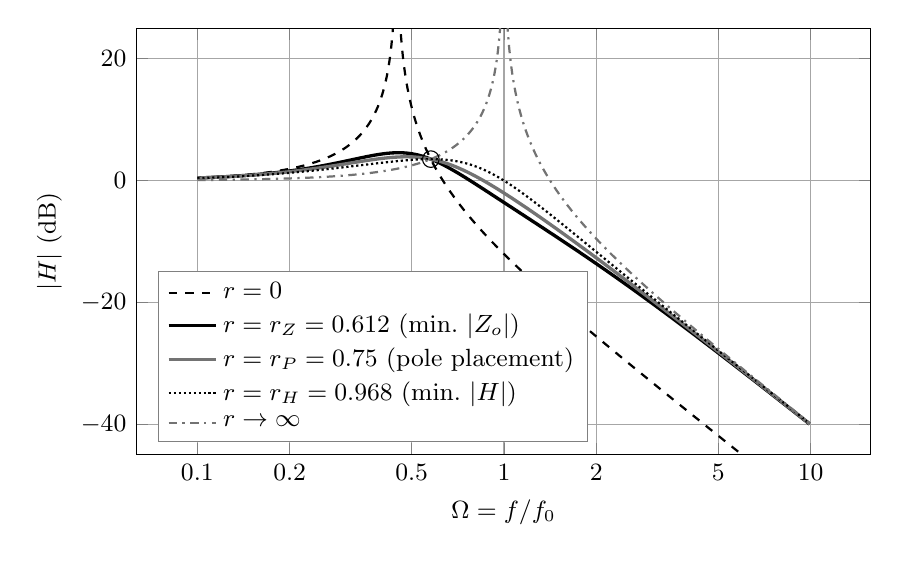
\begin{tikzpicture}
\begin{semilogxaxis}[bode, xlabel={$\Omega = f/f_0$}, ylabel={$|H|$ (dB)},
  domain=0.1:10, samples=600, ymin=-45, ymax=25, restrict y to domain=-80:80,
  xtick={0.1,0.2,0.5,1,2,5,10}, xticklabels={0.1,0.2,0.5,1,2,5,10},
  legend pos=south west]
  \addplot[l2] {dB(Hzero(x,4))};          \addlegendentry{$r = 0$}
  \addplot[l1] {dB(Hmag(x,4,rZ(4)))};     \addlegendentry{$r = r_Z = 0.612$ (min.~$|Z_o|$)}
  \addplot[l3] {dB(Hmag(x,4,rP(4)))};     \addlegendentry{$r = r_P = 0.75$ (pole placement)}
  \addplot[l4] {dB(Hmag(x,4,rH(4)))};     \addlegendentry{$r = r_H = 0.968$ (min.~$|H|$)}
  \addplot[l5] {dB(Hinf(x))};             \addlegendentry{$r \rightarrow \infty$}
  \addplot[only marks, mark=o, mark size=3pt, black] coordinates {(0.5774, 3.522)};
\end{semilogxaxis}
\end{tikzpicture}
\caption{$|H(j\Omega)|$ for $n = 4$ and several values of $r = R_2/R_0$. All curves pass
through the point $\Omega_m = \sqrt{2/(2+n)} = 0.577$, $|H| = (2+n)/n = 1.5$
(\SI{3.5}{\decibel}), marked by the circle.}
\label{fig:Hn4}
\end{figure}

\begin{figure}[htb]
\centering
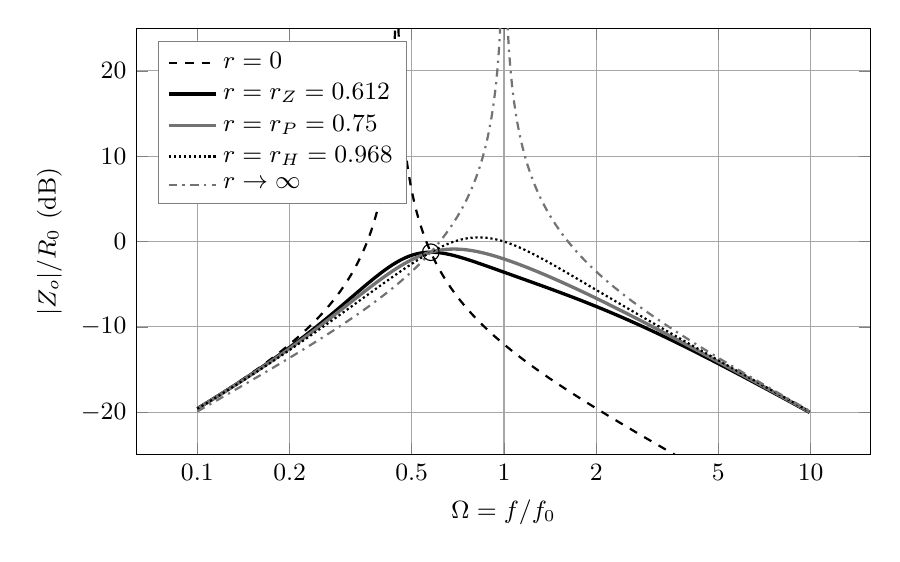
\begin{tikzpicture}
\begin{semilogxaxis}[bode, xlabel={$\Omega = f/f_0$}, ylabel={$|Z_o|/R_0$ (dB)},
  domain=0.1:10, samples=600, ymin=-25, ymax=25, restrict y to domain=-80:80,
  xtick={0.1,0.2,0.5,1,2,5,10}, xticklabels={0.1,0.2,0.5,1,2,5,10},
  legend pos=north west]
  \addplot[l2] {dB(x*Hzero(x,4))};          \addlegendentry{$r = 0$}
  \addplot[l1] {dB(x*Hmag(x,4,rZ(4)))};     \addlegendentry{$r = r_Z = 0.612$}
  \addplot[l3] {dB(x*Hmag(x,4,rP(4)))};     \addlegendentry{$r = r_P = 0.75$}
  \addplot[l4] {dB(x*Hmag(x,4,rH(4)))};     \addlegendentry{$r = r_H = 0.968$}
  \addplot[l5] {dB(x*Hinf(x))};             \addlegendentry{$r \rightarrow \infty$}
  \addplot[only marks, mark=o, mark size=3pt, black] coordinates {(0.5774, -1.249)};
\end{semilogxaxis}
\end{tikzpicture}
\caption{$|Z_o(j\Omega)|/R_0$ for $n = 4$. The common point is at $\Omega_m = 0.577$,
$|Z_o|/R_0 = \sqrt{2(2+n)}/n = 0.866$ (\SI{-1.2}{\decibel}). The curve for $r = r_Z$ has
its maximum exactly there.}
\label{fig:Zn4}
\end{figure}

\subsection{Optimum for the output impedance (Erickson)}
\label{sec:optZo}

Imposing that the maximum of $|Z_o|$ falls at $\Omega_m$, i.e.\
$\partial |Z_o|^2/\partial\Omega = 0$ at $\Omega = \Omega_m$, gives the classical result
\cite{Erickson1999,EricksonBook}
\begin{equation}
r_Z = \frac{R_{2,Z}}{R_0} = \sqrt{\frac{(2+n)(4+3n)}{2 n^2 (4+n)}}, \qquad
\left.\frac{\|Z_o\|_\infty}{R_0}\right|_{r_Z} = \frac{\sqrt{2(2+n)}}{n},
\label{eq:rZ}
\end{equation}
where $\|Z_o\|_\infty$ denotes the peak over frequency. This is the choice that minimises
the peak output impedance and is the relevant one when the concern is the interaction
with the load (load current steps, constant-power loads).

\subsection{Optimum for the voltage transfer function}
\label{sec:optH}

Since the curves of $|H|$ share the same crossing point, the same reasoning applied to
$|H|^2$ (Appendix~\ref{app:deriv}) gives
\begin{equation}
r_H = \frac{R_{2,H}}{R_0} = \frac{\sqrt{(1+n)(2+n)/2}}{n}, \qquad
\left.\|H\|_\infty\right|_{r_H} = \frac{2+n}{n}.
\label{eq:rH}
\end{equation}
This minimises the amplification of any component of the bridge voltage near the
resonance and the resonant peak seen by the current regulator. $r_H$ is always larger
than $r_Z$ (by a factor $\sqrt{(1+n)(4+n)/(4+3n)}$, i.e.\ $1.1$--$2$ for $n = 0.5$--$8$).

\subsection{Pole placement: real pole at \texorpdfstring{$\omega_0$}{w0}}
\label{sec:optP}

A third closed-form choice follows from factorising $D(p)$. For
\begin{equation}
r_P = \frac{2+n}{2n}
\label{eq:rP}
\end{equation}
one has $D(-1) = 2 + n - 2 n r_P = 0$, so that $p = -1$ (i.e.\ $s = -\omega_0$) is a
real pole and
\begin{equation}
D(p) = (1 + p)\left[1 + \frac{n}{2}\,p + \frac{2+n}{2}\,p^2\right],
\qquad
\omega_n = \omega_0 \sqrt{\frac{2}{2+n}} = \omega_0 \Omega_m,
\qquad
\zeta = \frac{n}{2\sqrt{2(2+n)}}.
\label{eq:zetaP}
\end{equation}
The complex pair has its natural frequency at the crossing point and a damping ratio that
is close to the maximum achievable with the branch (within \SI{7}{\percent} of it for
$n \le 4$, see Appendix~\ref{app:deriv}). $r_P$ lies between $r_Z$ and $r_H$ for every $n$, so it is a good single
compromise; the corresponding metrics are within a few percent of both optima.

\subsection{Summary table and choice of \texorpdfstring{$n$}{n}}

Table~\ref{tab:design} collects the three choices. The numbers were verified numerically
(peak search over frequency and over $r$, roots of $D(p)$, step response of $H$).

\begin{table}[htb]
\centering
\small
\caption{Closed-form design values of the damping branch versus $n = C_2/C_1$.
$r = R_2/R_0$. $\|Z_o\|_\infty$ is given for $r_Z$, $\|H\|_\infty$ for $r_H$, $\zeta$ and
the step overshoot of $v_o$ (step of $\overline{v_b}$) for $r_P$. $\Omega_m = f_m/f_0$ is
the frequency of the common point, $f_{low}/f_0 = 1/\sqrt{1+n}$ is the resonance of the
$L$--$(C_1+C_2)$ pair.}
\begin{tabular}{@{}S[table-format=1.1] S[table-format=1.3] S[table-format=1.3] S[table-format=1.3] S[table-format=1.3] S[table-format=1.3] S[table-format=1.3] S[table-format=2.0] S[table-format=1.3] S[table-format=1.3]@{}}
\toprule
{$n$} & {$r_Z$} & {$\dfrac{\|Z_o\|_\infty}{R_0}$} & {$r_H$} & {$\|H\|_\infty$} & {$r_P$} & {$\zeta_P$} & {OS (\%)} & {$\Omega_m$} & {$\dfrac{f_{low}}{f_0}$} \\
\midrule
0.5 & 2.472 & 4.472 & 2.739 & 5.000 & 2.500 & 0.112 & 80 & 0.894 & 0.816 \\
1   & 1.449 & 2.449 & 1.732 & 3.000 & 1.500 & 0.204 & 68 & 0.816 & 0.707 \\
2   & 0.913 & 1.414 & 1.225 & 2.000 & 1.000 & 0.354 & 53 & 0.707 & 0.577 \\
3   & 0.718 & 1.054 & 1.054 & 1.667 & 0.833 & 0.474 & 44 & 0.632 & 0.500 \\
4   & 0.612 & 0.866 & 0.968 & 1.500 & 0.750 & 0.577 & 38 & 0.577 & 0.447 \\
6   & 0.494 & 0.667 & 0.882 & 1.333 & 0.667 & 0.750 & 30 & 0.500 & 0.378 \\
8   & 0.427 & 0.559 & 0.839 & 1.250 & 0.625 & 0.894 & 25 & 0.447 & 0.333 \\
\bottomrule
\end{tabular}
\label{tab:design}
\end{table}

The table shows the trade-off governed by $n$. Increasing $n$ lowers both peaks roughly as
$1/n$ and raises the damping ratio, but the returns diminish above $n \approx 4$ while the
capacitor volume, the low-frequency corner shift and -- as shown in
Section~\ref{sec:losses} -- the losses in $R_2$ with a slow-AC output all grow with $C_2$.
The usual recommendation is:
\begin{itemize}[nosep]
\item $n = 4$ (or more) when the output is DC and the only concern is the resonance:
      $\|H\|_\infty \le \SI{3.5}{\decibel}$, $\|Z_o\|_\infty < R_0$, $\zeta \approx 0.6$;
\item $n = 2$--$3$ when the output carries slow AC or fast voltage slews, so that the
      reactive current $2\pi f_{ac} C_2 V_{ac}$ through $R_2$ stays acceptable:
      $\|H\|_\infty \le \SI{6}{\decibel}$, $\zeta \approx 0.35$--$0.47$;
\item $n = 1$ only when $C_2$ is very expensive (film at high voltage): the peaks are
      still $\SI{9.5}{\decibel}$ and $2.45 R_0$, acceptable for many control designs but
      not for a demanding load interaction.
\end{itemize}
Fig.~\ref{fig:Zn} shows $|Z_o|$ at the respective optimum for several $n$.

\begin{figure}[htb]
\centering
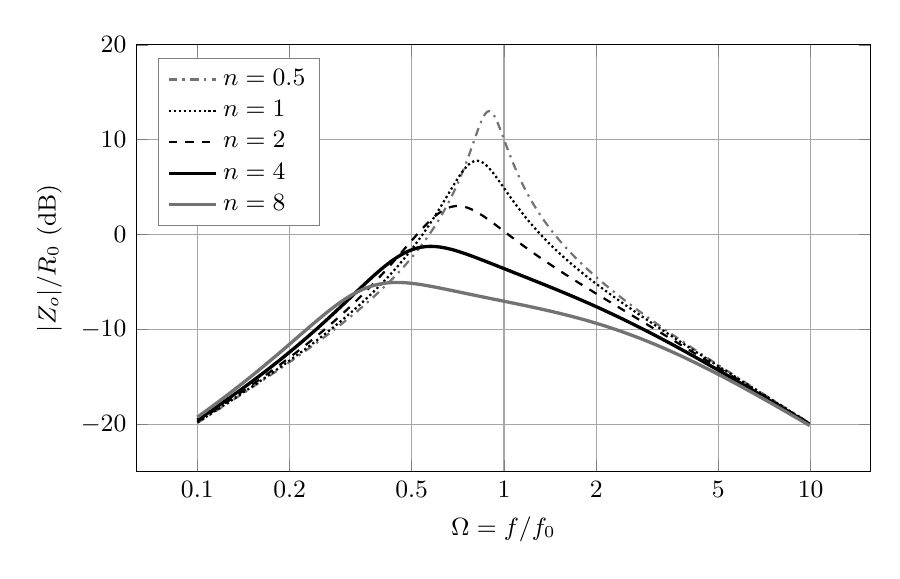
\begin{tikzpicture}
\begin{semilogxaxis}[bode, xlabel={$\Omega = f/f_0$}, ylabel={$|Z_o|/R_0$ (dB)},
  domain=0.1:10, samples=600, ymin=-25, ymax=20, restrict y to domain=-80:80,
  xtick={0.1,0.2,0.5,1,2,5,10}, xticklabels={0.1,0.2,0.5,1,2,5,10},
  legend pos=north west]
  \addplot[l5] {dB(x*Hmag(x,0.5,rZ(0.5)))};  \addlegendentry{$n = 0.5$}
  \addplot[l4] {dB(x*Hmag(x,1,rZ(1)))};      \addlegendentry{$n = 1$}
  \addplot[l2] {dB(x*Hmag(x,2,rZ(2)))};      \addlegendentry{$n = 2$}
  \addplot[l1] {dB(x*Hmag(x,4,rZ(4)))};      \addlegendentry{$n = 4$}
  \addplot[l3] {dB(x*Hmag(x,8,rZ(8)))};      \addlegendentry{$n = 8$}
\end{semilogxaxis}
\end{tikzpicture}
\caption{$|Z_o|/R_0$ with $r = r_Z$ for several capacitance ratios $n$. The peak is
$\sqrt{2(2+n)}/n$ and occurs at $\Omega_m = \sqrt{2/(2+n)}$.}
\label{fig:Zn}
\end{figure}

\subsection{Sensitivity to the value of \texorpdfstring{$R_2$}{R2}}

$R_2$ is never exactly at the design value: resistor tolerance, temperature coefficient,
the ESR of $C_2$ (which adds to $R_2$ and changes with temperature and ageing, especially
for electrolytic capacitors) and the series resistance of the connections all contribute.
Fig.~\ref{fig:sens} gives the peak of $|Z_o|$, normalised to its minimum, as a function of
$R_2/R_{2,Z}$. The curve is flat around the optimum: a $\pm\SI{25}{\percent}$ error costs
less than \SI{10}{\percent} (\SI{0.8}{\decibel}) of peak impedance; a factor of two costs
about \SI{50}{\percent} (\SI{3.5}{\decibel}). The design therefore tolerates the normal
spread of $R_2$ and of the ESR, provided that the nominal value is chosen at the centre of
the expected range and not at one extreme. Because $r_Z < r_P < r_H$, a value of $R_2$
anywhere between $r_Z R_0$ and $r_H R_0$ keeps all three metrics within a few percent of
their respective optima; if the ESR of $C_2$ is uncertain it is preferable to design the
external resistor so that the sum lands in this window.

\begin{figure}[htb]
\centering
\begin{tikzpicture}
\begin{semilogxaxis}[bode, xlabel={$R_2/R_{2,Z}$}, ylabel={$\|Z_o\|_\infty / \|Z_o\|_{\infty,\min}$},
  ymin=1, ymax=4,
  xtick={0.1,0.2,0.5,1,2,5,10}, xticklabels={0.1,0.2,0.5,1,2,5,10},
  legend style={at={(0.5,0.97)}, anchor=north, font=\small, fill=white, draw=black!50}]
  \addplot[l4] table[x=ratio, y=n1] {\senstable}; \addlegendentry{$n = 1$}
  \addplot[l2] table[x=ratio, y=n2] {\senstable}; \addlegendentry{$n = 2$}
  \addplot[l1] table[x=ratio, y=n4] {\senstable}; \addlegendentry{$n = 4$}
  \addplot[l3] table[x=ratio, y=n8] {\senstable}; \addlegendentry{$n = 8$}
\end{semilogxaxis}
\end{tikzpicture}
\caption{Sensitivity of the peak output impedance to the value of $R_2$, relative to the
optimum $R_{2,Z}$, for several $n$.}
\label{fig:sens}
\end{figure}

\subsection{Time-domain response}

Fig.~\ref{fig:step} shows the response of $v_o$ to a unit step of $\overline{v_b}$ for the
$r_Z$ designs and for the $r_P$ design with $n = 4$; time is normalised to $1/\omega_0$.
The overshoot (Table~\ref{tab:design}) is larger than the damping ratio alone would
suggest, because of the zero at $\Omega_z = 1/(n r)$ in $H(s)$: the branch feeds the
initial part of the step forward through $R_2$. The response settles (\SI{2}{\percent}) within
about $\omega_0 t \approx 15$--$25$, i.e.\ two to four periods of $f_0$ for $n = 2$--$4$,
against hundreds of periods for the undamped filter. In a closed-loop system the reference is rate-limited or shaped by the regulator,
so this overshoot is rarely reached; the response to a load current step, governed by
$Z_o$, is the more relevant transient and is bounded by $\|Z_o\|_\infty \Delta i_o$.

\begin{figure}[htb]
\centering
\begin{tikzpicture}
\begin{axis}[width=0.9\textwidth, height=7cm, grid=both,
  major grid style={black!35}, minor grid style={black!12},
  xlabel={$\omega_0 t$}, ylabel={$v_o/\Delta\overline{v_b}$},
  xmin=0, xmax=25, ymin=0, ymax=2.0, legend pos=north east,
  tick label style={font=\small}, label style={font=\small},
  legend style={font=\small, fill=white, draw=black!50}, legend cell align=left]
  \addplot[l4] table[x=t, y=n1] {\steptable};   \addlegendentry{$n = 1$, $r_Z$}
  \addplot[l2] table[x=t, y=n2] {\steptable};   \addlegendentry{$n = 2$, $r_Z$}
  \addplot[l1] table[x=t, y=n4] {\steptable};   \addlegendentry{$n = 4$, $r_Z$}
  \addplot[l3] table[x=t, y=n8] {\steptable};   \addlegendentry{$n = 8$, $r_Z$}
  \addplot[l5] table[x=t, y=n4p] {\steptable};  \addlegendentry{$n = 4$, $r_P$}
\end{axis}
\end{tikzpicture}
\caption{Response of the output voltage to a unit step of the average bridge voltage
(unloaded filter), for the designs of Table~\ref{tab:design}.}
\label{fig:step}
\end{figure}

% =====================================================================
\section{Design criteria for the output filter of a full bridge}
\label{sec:criteria}
% =====================================================================

\subsection{Ripple source: unipolar PWM}
\label{sec:pwm}

With unipolar voltage switching and a modulation index $m$ that varies slowly compared
with the carrier (quasi-static approximation, valid for $f_{ac} \ll f_{sw}$), the bridge
output is a pulse train of amplitude $V_{dc}$, frequency $f_r = 2 f_{sw}$ and duty
ratio $|m|$, with average $m V_{dc}$. Its Fourier series is
\begin{equation}
v_b(t) = m V_{dc} + \sum_{k=1}^{\infty} \hat V_k \cos(2\pi k f_r t + \varphi_k), \qquad
\hat V_k = \frac{2 V_{dc}}{k\pi}\,\bigl|\sin(k\pi |m|)\bigr|.
\label{eq:pwm}
\end{equation}
The first harmonic is maximum at $|m| = 0.5$, where $\hat V_1 = 2V_{dc}/\pi = 0.637\,V_{dc}$
and the second harmonic vanishes; the second harmonic is maximum ($V_{dc}/\pi$) at
$|m| = 0.25$ and $0.75$. For a sinusoidal output the same expressions hold instant by
instant, so the worst case is always $\hat V_1 = 2V_{dc}/\pi$ at $f_{r,\min}$
\cite{HolmesLipo,Mohan}.

The inductor current ripple, with the capacitor voltage taken as constant over one
ripple period, is
\begin{equation}
\Delta I_{L,pp} = \frac{|m|(1 - |m|)\,V_{dc}}{2 f_{sw} L} \le \frac{V_{dc}}{8 f_{sw} L},
\label{eq:dIL}
\end{equation}
triangular, with rms value $\Delta I_{L,pp}/(2\sqrt 3)$. This current flows almost
entirely into $C_1$ (the branch $C_2$--$R_2$ is resistive and much larger in impedance
than $C_1$ at $f_r$), so the peak-to-peak capacitor voltage ripple is
\begin{equation}
\Delta V_{o,pp} \simeq \frac{\Delta I_{L,pp}}{8 f_r C_1}
\qquad\text{or, from the first harmonic,}\qquad
\Delta V_{o,pp} \simeq 2\,\hat V_1\,|H(j 2\pi f_r)| \simeq 2\,\hat V_1 \left(\frac{f_0}{f_r}\right)^2 .
\label{eq:dVo}
\end{equation}
The two estimates agree within a few percent when $f_r \ge 5 f_0$.

\subsection{Design procedure}
\label{sec:procedure}

\begin{enumerate}[leftmargin=*]
\item \textbf{Inputs.} $V_{dc}$, rated current $I_n$, switching frequency range
      (worst case $f_{sw,\min}$), modulation type, output ripple specification
      $\Delta V_{o,pp}$ (or a load current ripple, converted through the load impedance at
      $f_r$), maximum output fundamental $f_{ac}$ and amplitude $\hat V_{ac}$, maximum
      voltage slew rate $(dv_o/dt)_{\max}$, load model ($L_\ell$, $R_\ell$ or a
      constant-power load $P$), required current-loop bandwidth $f_c$.

\item \textbf{Resonance frequency $f_0$.} From the ripple specification and
      \eqref{eq:dVo}, using the $-40$ dB/dec asymptote, which the branch does not alter,
      \begin{equation}
      f_0 \le f_{r,\min}\sqrt{\frac{\Delta V_{o,pp}}{2 \hat V_1}}
          = f_{r,\min}\sqrt{\frac{\pi\,\Delta V_{o,pp}}{4 V_{dc}}}.
      \label{eq:f0max}
      \end{equation}
      From the control side, the regulator crossover should satisfy $f_c \le f_0/5$ for a
      filter damped as in Table~\ref{tab:design} (resonant peak $\le \SI{6}{\decibel}$ and
      phase lag of $H$ below about \ang{15} at $f_c$). Both constraints define a window
      for $f_0$; with $f_{sw,\min} = \SI{1}{\kilo\hertz}$ and a ripple of
      \SI{1}{\percent} the window is roughly $f_0 \approx \SIrange{120}{180}{\hertz}$,
      which caps the current-loop bandwidth at some \SIrange{25}{35}{\hertz}. Keep $f_0$
      (and $f_{low} = f_0/\sqrt{1+n}$) away from the DC-link ripple frequency
      (\SI{300}{\hertz} for a six-pulse supply) and from $f_{ac}$ and its low harmonics.

\item \textbf{Inductor $L$.} From \eqref{eq:dIL}, limiting the ripple current to a
      fraction $\delta$ (typically $0.1$--$0.2$) of $I_n$ at $f_{sw,\min}$,
      $L \ge V_{dc}/(8 f_{sw,\min}\,\delta I_n)$. Check that the reactive drop
      $2\pi f_{ac} L I_n$ at the output fundamental is a small fraction of $V_{dc}$ and that
      the core is suitable for the combination of the DC/slow-AC bias and the
      \SIrange{2}{20}{\kilo\hertz} ripple.

\item \textbf{Capacitor $C_1$.} $C_1 = 1/(\omega_0^2 L)$; then $R_0 = \sqrt{L/C_1}$. The
      ripple current of $C_1$ is $\approx \Delta I_{L,pp}/(2\sqrt 3)$ at $f_r$ plus the
      reactive current $2\pi f_{ac} C_1 \hat V_{ac}/\sqrt 2$ at the output fundamental;
      a film (MKP) capacitor is the natural choice, with ESL low enough to keep its series
      resonance above $f_{r,\max}$.

\item \textbf{Ratio $n$ and capacitor $C_2$.} Choose $n$ from Table~\ref{tab:design}
      and the loss considerations of Section~\ref{sec:losses}; $C_2 = n C_1$. $C_2$ must
      withstand the full output voltage (DC bias plus overshoot); its ripple current is
      small at $f_r$ but equal to $2\pi f_{ac} C_2 \hat V_{ac}/\sqrt 2$ at the output
      fundamental and to $C_2\,dv_o/dt$ during slews.

\item \textbf{Resistor $R_2$.} $R_2 = r R_0$ with $r$ between $r_Z$ and $r_H$
      (Table~\ref{tab:design}); $r_P$ is a good default. Subtract the ESR of $C_2$ (and
      of its series/parallel arrangement) from the external resistor. The resistor must be
      non-inductive: its inductance $L_{R2}$ should satisfy
      $2\pi f_{r,\max} L_{R2} \ll R_2$ (for $R_2 = \SI{1}{\ohm}$ and
      $f_{r,\max} = \SI{20}{\kilo\hertz}$ this means well below \SI{8}{\micro\henry}, i.e.\
      a bifilar or thick-film construction).

\item \textbf{Load interaction.} Compare $\|Z_o\|_\infty$ with the load impedance in the
      band around $f_m$. For a passive $L_\ell$--$R_\ell$ load there is no stability
      issue; for a regulated converter drawing power $P$ at voltage $V_o$ require
      $\|Z_o\|_\infty \le \tfrac12\,V_o^2/P$ (\SI{6}{\decibel} margin on the Middlebrook
      criterion \cite{Middlebrook1976,Feng2002}), or apply the full impedance-ratio
      criterion with the measured or modelled input impedance of the load.

\item \textbf{Losses and ratings} (Section~\ref{sec:losses}).

\item \textbf{Verification.} Time-domain simulation (PLECS, Simscape) of the bridge with
      the real PWM, including the ESR/ESL of the capacitors and the inductor winding
      resistance, at $f_{sw,\min}$ and $f_{sw,\max}$, with $m = 0.5$ and with the slow-AC
      output at full amplitude; then measurement of $Z_o$ on the hardware with a
      frequency-response analyser or by a load current step.
\end{enumerate}

\subsection{Losses in the damping resistor and component ratings}
\label{sec:losses}

The current in the branch has three origins, which add in mean square.

\paragraph{Ripple at $f_r$.} The capacitor voltage ripple $\hat V_{o,k}$ at $k f_r$ drives
the branch through the impedance $R_2 + 1/(j 2\pi k f_r C_2)$, which is practically
equal to $R_2$:
\begin{equation}
P_{R2,r} \simeq \sum_k \frac{\hat V_{o,k}^2}{2 R_2}, \qquad
\hat V_{o,k} \simeq \hat V_k\,|H(j 2\pi k f_r)|.
\end{equation}
Because $\hat V_{o,k}$ is already attenuated by the filter this term is small (a few watts
to a few tens of watts at high power) and decreases with $f_{sw}$.

\paragraph{Slow-AC output.} A sinusoidal output $\hat V_{ac}$ at $f_{ac}$ drives a
reactive current through $C_2$, which necessarily flows in $R_2$:
\begin{equation}
I_{2,ac} = \frac{\hat V_{ac}}{\sqrt 2}\,\frac{\omega_{ac} C_2}{\sqrt{1 + (\omega_{ac} R_2 C_2)^2}}
\simeq \frac{\hat V_{ac}}{\sqrt 2}\,\omega_{ac} C_2, \qquad
P_{R2,ac} = I_{2,ac}^2 R_2 .
\label{eq:Pac}
\end{equation}
This term grows with $f_{ac}^2$, $\hat V_{ac}^2$ and $C_2^2 R_2 \propto n^2 r$; it is
usually the dominant loss when the output is not pure DC, and it is the reason for
limiting $n$ in slow-AC applications. The same current also loads $C_2$ (ripple current
rating at low frequency, where electrolytic capacitors are derated).

\paragraph{Voltage slews and steps.} During a controlled slew the branch carries
$i_2 \simeq C_2\,dv_o/dt$ and dissipates $R_2 i_2^2$. For an ideal step $\Delta V$ of the
output voltage, the energy dissipated in $R_2$ is $\tfrac12 C_2 \Delta V^2$ independently
of $R_2$ (the energy stored in $C_2$ is dissipated once on charge and once on discharge);
with $N$ steps per second the average power is $\tfrac12 C_2 \Delta V^2 N$ and the
resistor also needs an adequate pulse rating. In practice the slew rate of the reference
should be limited so that $C_2\,(dv_o/dt)_{\max}$ stays within the continuous rating of
$R_2$ and $C_2$.

\paragraph{Ratings.} $R_2$: continuous power $\ge P_{R2,r} + P_{R2,ac} + P_{R2,slew}$
with margin, plus the pulse energy; low inductance. $C_1$: voltage $\ge V_{dc}$ times
the overshoot factor; rms current at $f_r$ from \eqref{eq:dIL}. $C_2$: voltage as $C_1$;
rms current from \eqref{eq:Pac} and the slews; if electrolytic, series connection with
balancing resistors and a check of the ESR range over temperature, since the ESR is part
of $R_2$. $L$: rated for $I_n$ plus half the ripple, with the core loss at $f_r$.

% =====================================================================
\section{Worked example}
\label{sec:example}
% =====================================================================

The data below are representative of the application described in
Section~\ref{sec:appdata}; they are assumptions to be replaced by the actual project
values in the MATLAB script of Appendix~\ref{app:matlab}.

\begin{table}[htb]
\centering
\small
\caption{Example specification (assumed)}
\begin{tabular}{@{}lll@{}}
\toprule
DC-link voltage & $V_{dc}$ & \SI{800}{\volt} \\
Rated output current & $I_n$ & \SI{500}{\ampere} \\
Switching frequency per leg & $f_{sw}$ & \SIrange{1}{10}{\kilo\hertz} (ripple $f_r$ \SIrange{2}{20}{\kilo\hertz}) \\
Modulation & & unipolar voltage switching \\
Output & & DC or sinusoidal up to $f_{ac} = \SI{5}{\hertz}$, $\hat V_{ac} \le \SI{400}{\volt}$ \\
Load & $L_\ell$, $R_\ell$ & \SI{10}{\milli\henry}, \SI{0.1}{\ohm} \\
Output voltage ripple & $\Delta V_{o,pp}$ & $\le \SI{1}{\percent}\,V_{dc} = \SI{8}{\volt}$ at $f_{sw,\min}$, $m = 0.5$ \\
Inductor current ripple & $\delta$ & $\le \SI{20}{\percent}\,I_n$ at $f_{sw,\min}$ \\
Current-loop crossover & $f_c$ & $\approx \SI{30}{\hertz}$ \\
\bottomrule
\end{tabular}
\label{tab:spec}
\end{table}

\paragraph{Step 2 -- $f_0$.} $\hat V_1 = 2 \cdot 800/\pi = \SI{509}{\volt}$;
from \eqref{eq:f0max}, $f_0 \le 2000\sqrt{4/(2\cdot 509)} = \SI{177}{\hertz}$. The
control constraint gives $f_0 \ge 5 f_c = \SI{150}{\hertz}$. Target $f_0 \approx \SI{175}{\hertz}$.

\paragraph{Step 3 -- $L$.} $L \ge 800/(8 \cdot 1000 \cdot 100) = \SI{1.0}{\milli\henry}$;
chosen $L = \SI{1.2}{\milli\henry}$, giving $\Delta I_{L,pp} = \SI{83}{\ampere}$
(\SI{17}{\percent}, \SI{24}{\ampere} rms) at \SI{1}{\kilo\hertz} and \SI{8.3}{\ampere}
at \SI{10}{\kilo\hertz}. The reactive drop at \SI{5}{\hertz} is
$2\pi\cdot 5\cdot 1.2\cdot 10^{-3}\cdot 500 = \SI{19}{\volt}$, negligible.

\paragraph{Step 4 -- $C_1$.} $C_1 = 1/(\omega_0^2 L) \to \SI{680}{\micro\farad}$ (film),
$f_0 = \SI{176}{\hertz}$, $R_0 = \SI{1.33}{\ohm}$. Ripple current \SI{24}{\ampere} rms at
\SI{2}{\kilo\hertz}; \SI{6}{\ampere} rms at \SI{5}{\hertz} with $\hat V_{ac} = \SI{400}{\volt}$.

\paragraph{Steps 5--6 -- branch.} Two designs are compared in Table~\ref{tab:example}:
$n = 4$ ($C_2 = \SI{2.7}{\milli\farad}$) and $n = 2$ ($C_2 = \SI{1.36}{\milli\farad}$),
both with $r = r_P$. The undamped filter with a winding resistance of \SI{5}{\milli\ohm}
is shown for reference. The load contributes no damping:
$|Z_\ell(j\omega_0)| = \SI{11}{\ohm}$ and its parallel-equivalent resistance is
\SI{1.2}{\kilo\ohm}, i.e.\ $Q_{load} \approx 900$.

\begin{table}[htb]
\centering
\small
\caption{Worked example: results (values computed with the script of Appendix~\ref{app:matlab})}
\footnotesize
\begin{tabular}{@{}lccc@{}}
\toprule
 & undamped & $n = 2$, $r = r_P$ & $n = 4$, $r = r_P$ \\
\midrule
$C_2$ & -- & \SI{1.36}{\milli\farad} & \SI{2.7}{\milli\farad} \\
$R_2$ (incl.\ ESR of $C_2$) & -- & \SI{1.33}{\ohm} & \SI{1.0}{\ohm} \\
$f_{low} = f_0/\sqrt{1+n}$ & -- & \SI{102}{\hertz} & \SI{79}{\hertz} \\
$f_m$ & -- & \SI{125}{\hertz} & \SI{102}{\hertz} \\
Complex poles & $\zeta \approx 0.002$ & \SI{125}{\hertz}, $\zeta = 0.35$ & \SI{102}{\hertz}, $\zeta = 0.58$ \\
$\|H\|_\infty$ & $\approx 266$ (\SI{48}{\decibel}) & 2.06 (\SI{6.3}{\decibel}) at \SI{114}{\hertz} & 1.57 (\SI{3.9}{\decibel}) at \SI{85}{\hertz} \\
$\|Z_o\|_\infty$ & $\approx \SI{350}{\ohm}$ & \SI{1.89}{\ohm} at \SI{130}{\hertz} & \SI{1.20}{\ohm} at \SI{121}{\hertz} \\
$|H|$ at \SI{2}{\kilo\hertz} / \SI{20}{\kilo\hertz} & $-42$ / \SI{-82}{\decibel} & $-42$ / \SI{-82}{\decibel} & $-42$ / \SI{-82}{\decibel} \\
$\Delta V_{o,pp}$ at \SI{2}{\kilo\hertz}, $m = 0.5$ & \SI{7.9}{\volt} & \SI{7.9}{\volt} & \SI{7.9}{\volt} \\
$|H|$, phase at \SI{30}{\hertz} & 1.03, \ang{-0.0} & 1.09, \ang{-1.1} & 1.14, \ang{-3.1} \\
Step overshoot / settling (\SI{2}{\percent}) & \SI{100}{\percent} / $\approx\SI{2}{\second}$ & \SI{53}{\percent} / \SI{14}{\milli\second} & \SI{38}{\percent} / \SI{12}{\milli\second} \\
$I_2$, $P_{R2}$ at \SI{2}{\kilo\hertz} (ripple) & -- & \SI{2.1}{\ampere}, \SI{6}{\watt} & \SI{2.8}{\ampere}, \SI{8}{\watt} \\
$I_2$, $P_{R2}$ at \SI{5}{\hertz}, $\hat V_{ac} = \SI{165}{\volt}$ & -- & \SI{5.0}{\ampere}, \SI{33}{\watt} & \SI{9.9}{\ampere}, \SI{98}{\watt} \\
$I_2$, $P_{R2}$ at \SI{5}{\hertz}, $\hat V_{ac} = \SI{400}{\volt}$ & -- & \SI{12.1}{\ampere}, \SI{193}{\watt} & \SI{24.1}{\ampere}, \SI{578}{\watt} \\
$I_2$, $P_{R2}$ at \SI{5}{\hertz}, $\hat V_{ac} = \SI{600}{\volt}$ & -- & \SI{18.1}{\ampere}, \SI{435}{\watt} & \SI{36.1}{\ampere}, \SI{1300}{\watt} \\
$\hat i_2$ for $dv_o/dt = \SI{18.8}{\kilo\volt\per\second}$ (\SI{600}{\volt} pk, \SI{5}{\hertz}) & -- & \SI{26}{\ampere} & \SI{51}{\ampere} \\
\bottomrule
\end{tabular}
\label{tab:example}
\end{table}

\paragraph{Discussion.} Both damped designs meet the ripple specification (the branch
does not change the attenuation at $f_r$) and reduce the resonant peak from
\SI{48}{\decibel} to \SIrange{4}{6}{\decibel}, so that a \SI{30}{\hertz} current loop can
be closed with the filter treated as a mild second-order lag. The $n = 4$ design is
better in every dynamic respect, but with a \SI{400}{\volt} sinusoidal output at
\SI{5}{\hertz} its damping resistor dissipates about \SI{0.6}{\kilo\watt} continuously,
three times more than the $n = 2$ design, and its branch carries \SI{24}{\ampere} rms
at \SI{5}{\hertz}, which an electrolytic $C_2$ tolerates less well than a film one.
For a predominantly DC output the $n = 4$ design is preferred; for continuous slow-AC
operation at large amplitude $n = 2$ (or $n = 3$) with a film $C_2$ is the better
compromise, unless the loss is accepted. In both cases $R_2$ should be a non-inductive
resistor of at least twice the computed continuous power, and the reference slew rate
should be limited so that $C_2\,dv_o/dt$ does not exceed the rms current rating of $C_2$.
Fig.~\ref{fig:example} shows $|H|$ of the three cases against the real frequency axis
together with the two ripple frequencies.

\begin{figure}[htb]
\centering
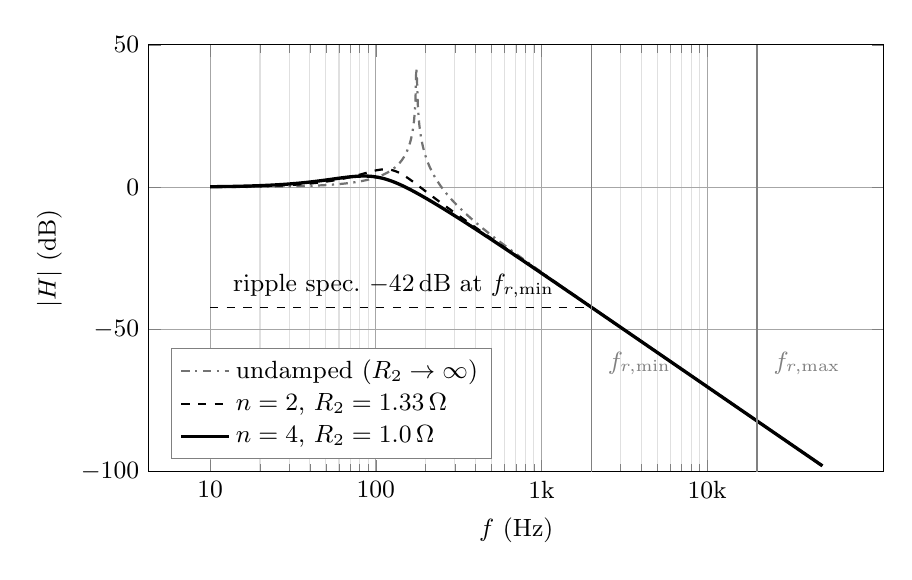
\begin{tikzpicture}
\begin{semilogxaxis}[bode, xlabel={$f$ (Hz)}, ylabel={$|H|$ (dB)},
  domain=10:50000, samples=800, ymin=-100, ymax=50, restrict y to domain=-120:120,
  xtick={10,100,1000,10000}, xticklabels={10,100,1k,10k},
  legend pos=south west]
  \addplot[l5] {dB(Hinf(x/176.2))};               \addlegendentry{undamped ($R_2 \rightarrow \infty$)}
  \addplot[l2] {dB(Hmag(x/176.2,2,1.0))};         \addlegendentry{$n = 2$, $R_2 = \SI{1.33}{\ohm}$}
  \addplot[l1] {dB(Hmag(x/176.2,4,0.75))};        \addlegendentry{$n = 4$, $R_2 = \SI{1.0}{\ohm}$}
  \draw[black!50, thin] (axis cs:2000,-100) -- (axis cs:2000,50);
  \node[black!50, font=\small, anchor=west] at (axis cs:2200,-62) {$f_{r,\min}$};
  \draw[black!50, thin] (axis cs:20000,-100) -- (axis cs:20000,50);
  \node[black!50, font=\small, anchor=west] at (axis cs:22000,-62) {$f_{r,\max}$};
  \draw[black, dashed, thin] (axis cs:10,-42.2) -- (axis cs:2000,-42.2);
  \node[font=\small, anchor=south west] at (axis cs:12,-42.2) {ripple spec.\ \SI{-42}{\decibel} at $f_{r,\min}$};
\end{semilogxaxis}
\end{tikzpicture}
\caption{Worked example: $|H|$ for the undamped filter and for the two damped designs
($L = \SI{1.2}{\milli\henry}$, $C_1 = \SI{680}{\micro\farad}$, $f_0 = \SI{176}{\hertz}$).
The undamped peak is limited by the parasitic resistances (here drawn without them).}
\label{fig:example}
\end{figure}

% =====================================================================
\section{Practical notes}
\label{sec:practical}
% =====================================================================

\begin{itemize}[leftmargin=*]
\item \textbf{Capacitor technology.} $C_1$ carries the ripple current at $f_r$ and must be
      a film capacitor with low ESL; $C_2$ carries little current at $f_r$ and can be an
      electrolytic bank (series-connected for $V_{dc} > \SI{400}{\volt}$, with balancing
      resistors) when the output is DC, whereas for continuous slow-AC output a film
      $C_2$ avoids the low-frequency ripple-current derating of electrolytics. The ESR of
      $C_2$ is part of $R_2$; with electrolytics it may be a substantial part, and its
      range over temperature and lifetime must be inside the flat region of
      Fig.~\ref{fig:sens}.
\item \textbf{Resistor construction.} $R_2$ must be non-inductive with respect to
      $f_{r,\max}$; wire-wound resistors of ordinary construction are not suitable. Thick-film
      on heatsink, bifilar or Ayrton-Perry wound resistors, or several resistors in
      parallel, are appropriate. Mount it with a thermal path sized for the slow-AC loss.
\item \textbf{Parasitics.} The ESR of $C_1$ adds a zero at $1/(2\pi\,\mathrm{ESR}\,C_1)$
      that flattens the $-40$ dB/dec asymptote to $-20$ dB/dec, and its ESL adds a series
      resonance above which the attenuation stops improving. Both must be above
      $f_{r,\max}$ with margin. The winding resistance of $L$ helps the damping only
      marginally and should not be relied upon.
\item \textbf{Low-frequency corner.} With $n = 4$ the response starts to deviate from
      unity at $f_0/\sqrt 5$; if the current loop or the slow-AC output needs a flat
      response up to a given frequency, check $|H|$ and $\arg H$ there rather than at $f_0$.
\item \textbf{DC-link ripple.} The DC-link ripple appears at the output multiplied by $m$
      and by $|H|$ at its frequency. If the six-pulse ripple at \SI{300}{\hertz} lies just
      above $f_0$, $|H|$ there is still only about \SI{-10}{\decibel} (example of
      Section~\ref{sec:example}); size the DC-link capacitor accordingly or move $f_0$
      lower.
\item \textbf{Protection.} On a crowbar or bypass event at the load, the filter capacitors
      discharge through the fault; $C_2$ discharges through $R_2$, which limits its
      contribution, while $C_1$ is limited only by the loop inductance. Consider this in
      the fault current budget and in the pulse rating of $R_2$.
\item \textbf{Measurement.} The most direct check on the hardware is the output impedance,
      measured by injecting a current at the output with the bridge in freewheeling or
      at zero modulation, or the response of $v_o$ to a load current step; the peak and
      its frequency should match $\|Z_o\|_\infty$ and $f_m$ of Table~\ref{tab:design}.
\end{itemize}

\section{Conclusions}

The $C_2$--$R_2$ branch in parallel with the filter capacitor is the passive damping
that best suits a high-current DC or slow-AC output filter: it dissipates nothing in DC,
leaves the \SI{-40}{\decibel\per decade} ripple attenuation untouched and damps the
resonance regardless of the load. Its design reduces to two dimensionless numbers. The
ratio $n = C_2/C_1$ sets the achievable peaks, $\|H\|_\infty = (2+n)/n$ and
$\|Z_o\|_\infty = R_0\sqrt{2(2+n)}/n$, at the frequency $f_0\sqrt{2/(2+n)}$; $n = 2$--$4$
is the practical range. The resistance $r = R_2/R_0$ is chosen between the Erickson
optimum $r_Z$ (minimum output impedance peak) and $r_H$ (minimum transfer-function peak),
the pole-placement value $r_P = (2+n)/(2n)$ being a convenient default; the result is
insensitive to $\pm\SI{25}{\percent}$ errors in $R_2$. The cost of the branch is the
capacitor $C_2$ and, when the output carries slow AC or fast slews, the reactive current
$2\pi f_{ac} C_2 \hat V_{ac}$ that flows through $R_2$, which must be included in the loss
budget and in the ratings of $R_2$ and $C_2$ and which limits $n$ in such applications.

\appendix

% =====================================================================
\section{Derivations}
\label{app:deriv}
% =====================================================================

\subsection{Shunt network and transfer functions}

With $Z_1 = 1/(sC_1)$ and $Z_2 = R_2 + 1/(sC_2) = (1 + sR_2C_2)/(sC_2)$,
\begin{equation}
Z_c = \frac{Z_1 Z_2}{Z_1 + Z_2}
    = \frac{\dfrac{1 + sR_2C_2}{s^2 C_1 C_2}}{\dfrac{(C_1 + C_2) + sR_2C_1C_2}{sC_1C_2}}
    = \frac{1 + sR_2C_2}{s\,[(C_1+C_2) + sR_2C_1C_2]},
\end{equation}
which is \eqref{eq:Zc} with $C_s = C_1C_2/(C_1+C_2)$. Then
\begin{equation}
H = \frac{Z_c}{sL + Z_c}
  = \frac{1 + sR_2C_2}{s^2 L\,[(C_1+C_2) + sR_2C_1C_2] + 1 + sR_2C_2},
\end{equation}
which is \eqref{eq:H}; $Z_o = sL Z_c/(sL + Z_c) = sL\,H$ and $Z_{in} = sL + Z_c$ follow
directly. With $s = p\,\omega_0$, $\omega_0^2 L C_1 = 1$, $\omega_0 R_0 C_1 = 1$,
$C_2 = nC_1$ and $R_2 = rR_0$:
\begin{align}
sR_2C_2 &= p\,\omega_0\, r R_0\, n C_1 = n r\, p, \\
s^2 L (C_1 + C_2) &= p^2\,\omega_0^2 L C_1 (1+n) = (1+n)\,p^2, \\
s^3 L R_2 C_1 C_2 &= p^3\,\omega_0^3 L C_1\, r R_0\, n C_1 = n r\, p^3 ,
\end{align}
giving \eqref{eq:D}--\eqref{eq:Hnorm}.

\subsection{Common point of the magnitude curves}

With $x = nr\Omega$, $A = 1 - (1+n)\Omega^2$, $B = 1 - \Omega^2$,
\begin{equation}
|H|^2 = \frac{1 + x^2}{A^2 + x^2 B^2}.
\end{equation}
$|H|^2$ is independent of $x$ if and only if $A^2 = B^2$; $A = B$ requires $n\Omega^2 = 0$,
so $A = -B$: $1 - (1+n)\Omega^2 = \Omega^2 - 1$, i.e.\ $\Omega_m^2 = 2/(2+n)$. There
$B = 1 - 2/(2+n) = n/(2+n)$ and $|H| = 1/|B| = (2+n)/n$, $|Z_o|/R_0 = \Omega_m |H| =
\sqrt{2/(2+n)}\,(2+n)/n = \sqrt{2(2+n)}/n$. For any $r$ the peak of a curve is at least
the value at the common point, so these are lower bounds on the achievable peaks.

\subsection{Optimum values of \texorpdfstring{$r$}{r}}

Let $G(\Omega) = |H|^2$ and $F(\Omega) = \Omega^2 |H|^2 = |Z_o|^2/R_0^2$. A curve whose
maximum lies at the common point satisfies $\partial G/\partial\Omega = 0$ (resp.\
$\partial F/\partial\Omega = 0$) at $\Omega = \Omega_m$. Carrying out the differentiation
of the rational functions and substituting $\Omega_m^2 = 2/(2+n)$ yields a single
equation in $r^2$ in each case, with the positive roots
\begin{equation}
r_Z^2 = \frac{6n^2 + 20n + 16}{4n^2(n+4)} = \frac{(2+n)(4+3n)}{2n^2(4+n)}, \qquad
r_H^2 = \frac{2n^2 + 6n + 4}{4n^2} = \frac{(1+n)(2+n)}{2n^2}.
\end{equation}
The first is Erickson's result \cite{Erickson1999}; both were checked numerically by a
direct minimisation of the peak over $r$ (Section~\ref{sec:theory}). Note that $r_H > r_Z$
for all $n > 0$: $r_H/r_Z = \sqrt{(1+n)(4+n)/(4+3n)}$, which grows slowly with $n$.

\subsection{Pole placement}

$D(p) = 1 + nr\,p + (1+n)\,p^2 + nr\,p^3$ has $p = -1$ as a root when
$1 - nr + (1+n) - nr = 0$, i.e.\ $r = r_P = (2+n)/(2n)$, for which $nr_P = (2+n)/2$.
Dividing by $(1+p)$,
\begin{equation}
D(p) = (1+p)\left(\frac{2+n}{2}\,p^2 + \frac{n}{2}\,p + 1\right),
\end{equation}
so the complex pair has $\omega_n/\omega_0 = \sqrt{2/(2+n)} = \Omega_m$ and
$2\zeta\,\omega_n/\omega_0 = n/(2+n)$, i.e.\ $\zeta = n/(2\sqrt{2(2+n)})$. Numerically
the damping ratio of the complex pair as a function of $r$ has its maximum slightly above
$r_P$ ($0.62$ against $0.58$ for $n = 4$, $0.37$ against $0.35$ for $n = 2$).

\subsection{Unipolar PWM pulse train}

For a constant modulation index $m > 0$ the leg voltages are $v_A = V_{dc}$ when the
carrier is below $m$ and $v_B = V_{dc}$ when it is below $-m$; the difference
$v_b = v_A - v_B$ equals $V_{dc}$ while the carrier lies between $-m$ and $m$ and is zero
otherwise. With a triangular carrier this happens once in every half carrier period, for
a fraction $m$ of it, so $v_b$ is a pulse train of period $1/(2f_{sw})$, amplitude
$V_{dc}$ and duty ratio $m$. Its Fourier coefficients are
$\hat V_k = (2V_{dc}/k\pi)|\sin(k\pi m)|$, which is \eqref{eq:pwm}; the result was checked
by FFT of the sampled waveform for $m = 0.5$ and $m = 0.25$.

% =====================================================================
\section{MATLAB script}
\label{app:matlab}
% =====================================================================

The script below (\texttt{damped\_lc\_filter.m}, Control System Toolbox) reproduces the
design procedure of Section~\ref{sec:procedure} and the numbers of
Section~\ref{sec:example}; the input block at the top is the only part to edit. It
builds $H(s)$, $Z_o(s)$, $Z_{in}(s)$ and the loaded transfer function, prints the
peaks, the poles and the loss estimates, sweeps $R_2$ around the optimum and plots the
frequency and step responses in grey scale.

\begin{lstlisting}
%% damped_lc_filter.m
% L - C1 - (C2 + R2) output filter of an IGBT full bridge (unipolar PWM).
% Companion of "Passively Damped LC Output Filter with R-C Damping Branch",
% Rev. 00, 2026-09-21.  Requires the Control System Toolbox.
clear; clc; close all

%% ---- Input data (edit) -------------------------------------------------
Vdc   = 800;          % DC-link voltage [V]
In    = 500;          % rated output current [A]
fsw   = [1e3 10e3];   % switching frequency range per leg [Hz]
dVpp  = 0.01*Vdc;     % output voltage ripple spec, peak-to-peak [V]
delta = 0.20;         % max inductor current ripple, fraction of In
fc    = 30;           % current-loop crossover [Hz]
fac   = 5;            % max output fundamental [Hz]
Vac   = 400;          % max slow-AC output amplitude [V peak]
dvdt  = 2*pi*fac*600; % max output voltage slew rate [V/s]
Lload = 10e-3;  Rload = 0.1;      % load model
n     = 4;            % C2/C1
crit  = 'P';          % 'Z' Erickson (min peak Zo), 'H' (min peak H), 'P' (pole at -w0)
L     = 1.2e-3;       % chosen inductor [H]   (see step 3)
C1    = 680e-6;       % chosen capacitor [F]  (see step 4)

%% ---- Step 2: resonance frequency window -------------------------------
fr    = 2*fsw;                      % ripple frequency (unipolar PWM)
V1    = 2*Vdc/pi;                   % worst-case first harmonic (m = 0.5)
f0max = min(fr)*sqrt(dVpp/(2*V1));  % from the -40 dB/dec asymptote
f0min = 5*fc;                       % from the control bandwidth
fprintf('f0 window: %.0f ... %.0f Hz\n', f0min, f0max);

%% ---- Step 3: inductor ---------------------------------------------------
Lmin  = Vdc/(8*min(fsw)*delta*In);
dIpp  = Vdc./(8*fsw*L);             % worst-case ripple (m = 0.5)
fprintf('L >= %.2f mH, chosen %.2f mH -> dI_pp = %.1f / %.1f A\n', ...
        Lmin*1e3, L*1e3, dIpp);

%% ---- Step 4: capacitor and base quantities ------------------------------
w0 = 1/sqrt(L*C1);  f0 = w0/(2*pi);  R0 = sqrt(L/C1);
fprintf('f0 = %.1f Hz, R0 = %.3f ohm\n', f0, R0);

%% ---- Steps 5-6: damping branch -----------------------------------------
rZ = sqrt((2+n)*(4+3*n)/(2*n^2*(4+n)));   % Erickson, min peak |Zo|
rH = sqrt((1+n)*(2+n)/2)/n;               % min peak |H|
rP = (2+n)/(2*n);                         % real pole at -w0
switch crit
    case 'Z', r = rZ;
    case 'H', r = rH;
    otherwise, r = rP;
end
C2 = n*C1;  R2 = r*R0;
fprintf('n = %g: rZ = %.3f, rH = %.3f, rP = %.3f -> R2 = %.3f ohm, C2 = %.2f mF\n', ...
        n, rZ, rH, rP, R2, C2*1e3);
fprintf('closed form: peak|Zo| = %.3f ohm (rZ), peak|H| = %.3f (rH), fm = %.1f Hz\n', ...
        R0*sqrt(2*(2+n))/n, (2+n)/n, f0*sqrt(2/(2+n)));

%% ---- Transfer functions -------------------------------------------------
s   = tf('s');
Zc  = (1 + s*R2*C2)/(s*((C1+C2) + s*R2*C1*C2));   % shunt network
H   = minreal(Zc/(s*L + Zc));                      % vo/vb, unloaded
Zo  = minreal(s*L*H);                              % output impedance
Zin = minreal(s*L + Zc);                           % seen by the bridge
Zl  = Rload + s*Lload;
Zcl = minreal(Zc*Zl/(Zc + Zl));
Hl  = minreal(Zcl/(s*L + Zcl));                    % vo/vb, loaded
Hund = 1/(1 + s^2*L*C1);                           % undamped reference

[gH, wH] = getPeakGain(H);   [gZ, wZ] = getPeakGain(Zo);
fprintf('peak|H| = %.3f (%.1f dB) at %.0f Hz; peak|Zo| = %.3f ohm at %.0f Hz\n', ...
        gH, 20*log10(gH), wH/(2*pi), gZ, wZ/(2*pi));
damp(H)                                            % poles, zeta, frequencies

%% ---- Ripple check -------------------------------------------------------
for k = 1:numel(fr)
    Hk  = abs(freqresp(H, 2*pi*fr(k)));
    Vo1 = V1*Hk;                                  % first harmonic at output
    w   = 2*pi*fr(k);
    I2  = Vo1/sqrt(2)/abs(R2 + 1/(1j*w*C2));      % branch current, rms
    fprintf('fr = %5.0f Hz: |H| = %.1f dB, dVo_pp = %.2f V (%.2f %%), I2 = %.2f A rms, P_R2 = %.1f W\n', ...
            fr(k), 20*log10(Hk), 2*Vo1, 200*Vo1/Vdc, I2, I2^2*R2);
end
fprintf('triangular estimate: dVo_pp = %.2f V at fr,min\n', dIpp(1)/(8*fr(1)*C1));

%% ---- Slow-AC and slew losses in R2 -------------------------------------
wac  = 2*pi*fac;
I2ac = Vac/sqrt(2)*wac*C2/sqrt(1 + (wac*R2*C2)^2);
I1ac = Vac/sqrt(2)*wac*C1;
fprintf('%g Hz, %g V pk: I2 = %.1f A rms -> P_R2 = %.0f W; I_C1 = %.1f A rms\n', ...
        fac, Vac, I2ac, I2ac^2*R2, I1ac);
fprintf('slew %.1f kV/s: i2 = %.0f A pk, %.1f kW in R2 during the slew\n', ...
        dvdt/1e3, C2*dvdt, (C2*dvdt)^2*R2/1e3);

%% ---- Low-frequency behaviour (control) ---------------------------------
for f = [fac fc 2*fc]
    h = freqresp(H, 2*pi*f);
    fprintf('f = %4.0f Hz: |H| = %.3f, phase = %.1f deg\n', f, abs(h), angle(h)*180/pi);
end

%% ---- Sensitivity of the peaks to R2 -------------------------------------
kk = logspace(-1, 1, 41);  pkZ = zeros(size(kk));  pkH = pkZ;
for i = 1:numel(kk)
    R2i = kk(i)*rZ*R0;
    Zci = (1 + s*R2i*C2)/(s*((C1+C2) + s*R2i*C1*C2));
    Hi  = minreal(Zci/(s*L + Zci));
    pkH(i) = getPeakGain(Hi);  pkZ(i) = getPeakGain(minreal(s*L*Hi));
end

%% ---- Plots (grey scale) -------------------------------------------------
fv = logspace(0, 5, 2000);  w = 2*pi*fv;
figure('Name', 'Voltage transfer function');
semilogx(fv, 20*log10(squeeze(abs(freqresp(Hund, w)))), '-.', 'Color', [.55 .55 .55], 'LineWidth', 1.2); hold on
semilogx(fv, 20*log10(squeeze(abs(freqresp(H, w)))),    'k-',  'LineWidth', 1.6);
semilogx(fv, 20*log10(squeeze(abs(freqresp(Hl, w)))),   'k--', 'LineWidth', 1.2);
xline(fr(1), ':', 'Color', [.4 .4 .4]); xline(fr(end), ':', 'Color', [.4 .4 .4]);
grid on; ylim([-100 50]); xlabel('f (Hz)'); ylabel('|H| (dB)');
legend('undamped', 'damped, unloaded', 'damped, loaded', 'Location', 'southwest');

figure('Name', 'Output impedance');
semilogx(fv, 20*log10(squeeze(abs(freqresp(Zo, w)))), 'k-', 'LineWidth', 1.6); hold on
semilogx(fv, 20*log10(abs(1j*w*L)), ':', 'Color', [.5 .5 .5]);
semilogx(fv, 20*log10(1./(w*C1)), ':', 'Color', [.5 .5 .5]);
grid on; xlabel('f (Hz)'); ylabel('|Z_o| (dB ohm)'); ylim([-40 20]);
legend('|Z_o|', '\omega L', '1/(\omega C_1)', 'Location', 'south');

figure('Name', 'Peak sensitivity');
semilogx(kk, pkZ/min(pkZ), 'k-', kk, pkH/min(pkH), 'k--', 'LineWidth', 1.4);
grid on; xlabel('R_2 / R_{2,Z}'); ylabel('peak / minimum peak');
legend('|Z_o|', '|H|', 'Location', 'north');

figure('Name', 'Step response');
[y, t] = step(H, 0.06);  [yl, tl] = step(Hl, 0.06);
plot(t*1e3, y, 'k-', tl*1e3, yl, 'k--', 'LineWidth', 1.4); grid on
xlabel('t (ms)'); ylabel('v_o / \Delta v_b'); legend('unloaded', 'loaded');
S = stepinfo(H);
fprintf('step: overshoot %.1f %%, settling (2 %%) %.1f ms\n', S.Overshoot, S.SettlingTime*1e3);
\end{lstlisting}

% =====================================================================
\begin{thebibliography}{99}
\raggedright
\small

\bibitem{Middlebrook1976}
R.~D. Middlebrook, ``Input filter considerations in design and application of switching
regulators,'' in \emph{Conf.\ Rec.\ IEEE Ind.\ Appl.\ Soc.\ Annu.\ Meeting}, Chicago,
IL, USA, Oct.\ 1976, pp.~366--382.

\bibitem{Middlebrook1978}
R.~D. Middlebrook, ``Design techniques for preventing input-filter oscillation in
switched-mode regulators,'' in \emph{Proc.\ Powercon~5}, San Francisco, CA, USA, May
1978, pp.~A3.1--A3.16.

\bibitem{Phelps1979}
T.~K. Phelps and W.~S. Tate, ``Optimizing passive input filter design,'' in \emph{Proc.\
Powercon~6}, May 1979, pp.~G1.1--G1.10.

\bibitem{Erickson1999}
R.~W. Erickson, ``Optimal single resistor damping of input filters,'' in \emph{Proc.\
IEEE Appl.\ Power Electron.\ Conf.\ Expo.\ (APEC)}, Dallas, TX, USA, Mar.\ 1999,
vol.~2, pp.~1073--1079.

\bibitem{EricksonBook}
R.~W. Erickson and D. Maksimovi\'c, \emph{Fundamentals of Power Electronics}, 2nd ed.
Norwell, MA, USA: Kluwer, 2001, ch.~10, ``Input filter design.''

\bibitem{Erich1992}
S.~Y. Erich and W.~M. Polivka, ``Input filter design criteria for current-programmed
regulators,'' \emph{IEEE Trans.\ Power Electron.}, vol.~7, no.~1, pp.~143--151, Jan.\
1992.

\bibitem{Vlatkovic1996}
V. Vlatkovi\'c, D. Borojevi\'c, and F.~C. Lee, ``Input filter design for power factor
correction circuits,'' \emph{IEEE Trans.\ Power Electron.}, vol.~11, no.~1,
pp.~199--205, Jan.\ 1996.

\bibitem{Feng2002}
X. Feng, J. Liu, and F.~C. Lee, ``Impedance specifications for stable DC distributed
power systems,'' \emph{IEEE Trans.\ Power Electron.}, vol.~17, no.~2, pp.~157--162,
Mar.\ 2002.

\bibitem{Riccobono2014}
A. Riccobono and E. Santi, ``Comprehensive review of stability criteria for DC power
distribution systems,'' \emph{IEEE Trans.\ Ind.\ Appl.}, vol.~50, no.~5,
pp.~3525--3535, Sep./Oct.\ 2014.

\bibitem{Cespedes2011}
M. Cespedes, L. Xing, and J. Sun, ``Constant-power load system stabilization by passive
damping,'' \emph{IEEE Trans.\ Power Electron.}, vol.~26, no.~7, pp.~1832--1836, Jul.\
2011.

\bibitem{Liserre2005}
M. Liserre, F. Blaabjerg, and S. Hansen, ``Design and control of an LCL-filter-based
three-phase active rectifier,'' \emph{IEEE Trans.\ Ind.\ Appl.}, vol.~41, no.~5,
pp.~1281--1291, Sep./Oct.\ 2005.

\bibitem{PenaAlzola2013}
R. Pe\~na-Alzola, M. Liserre, F. Blaabjerg, R. Sebasti\'an, J. Dannehl, and F.~W. Fuchs,
``Analysis of the passive damping losses in LCL-filter-based grid converters,''
\emph{IEEE Trans.\ Power Electron.}, vol.~28, no.~6, pp.~2642--2646, Jun.\ 2013.

\bibitem{Wu2013}
W. Wu, Y. He, T. Tang, and F. Blaabjerg, ``A new design method for the passive damped
LCL and LLCL filter-based single-phase grid-tied inverter,'' \emph{IEEE Trans.\ Ind.\
Electron.}, vol.~60, no.~10, pp.~4339--4350, Oct.\ 2013.

\bibitem{HolmesLipo}
D.~G. Holmes and T.~A. Lipo, \emph{Pulse Width Modulation for Power Converters:
Principles and Practice}. Piscataway, NJ, USA: IEEE Press/Wiley, 2003.

\bibitem{Mohan}
N. Mohan, T.~M. Undeland, and W.~P. Robbins, \emph{Power Electronics: Converters,
Applications, and Design}, 3rd ed. Hoboken, NJ, USA: Wiley, 2003, ch.~8.

\end{thebibliography}

\end{document}
